\section*{ПРИЛОЖЕНИЕ A}
\addcontentsline{toc}{section}{ПРИЛОЖЕНИЕ A}

\begin{figure}[h]
	\centering
	\captionsetup{justification=centering}
	
\includegraphics[width=150mm]{img/slide1.png}
	\caption{Титульный слайд (слайд 1)}
	\label{fig:slide-1}
\end{figure}

\begin{figure}[h]
	\centering
	\captionsetup{justification=centering}
	
\includegraphics[width=150mm]{img/slide2.png}
	\caption{Цель работы (слайд 2)}
	\label{fig:slide-2}
\end{figure}

\begin{figure}[h]
	\centering
	\captionsetup{justification=centering}
	
\includegraphics[width=150mm]{img/slide3.png}
	\caption{Задачи работы (слайд 3)}
	\label{fig:slide-3}
\end{figure}

\begin{figure}[h]
	\centering
	\captionsetup{justification=centering}
	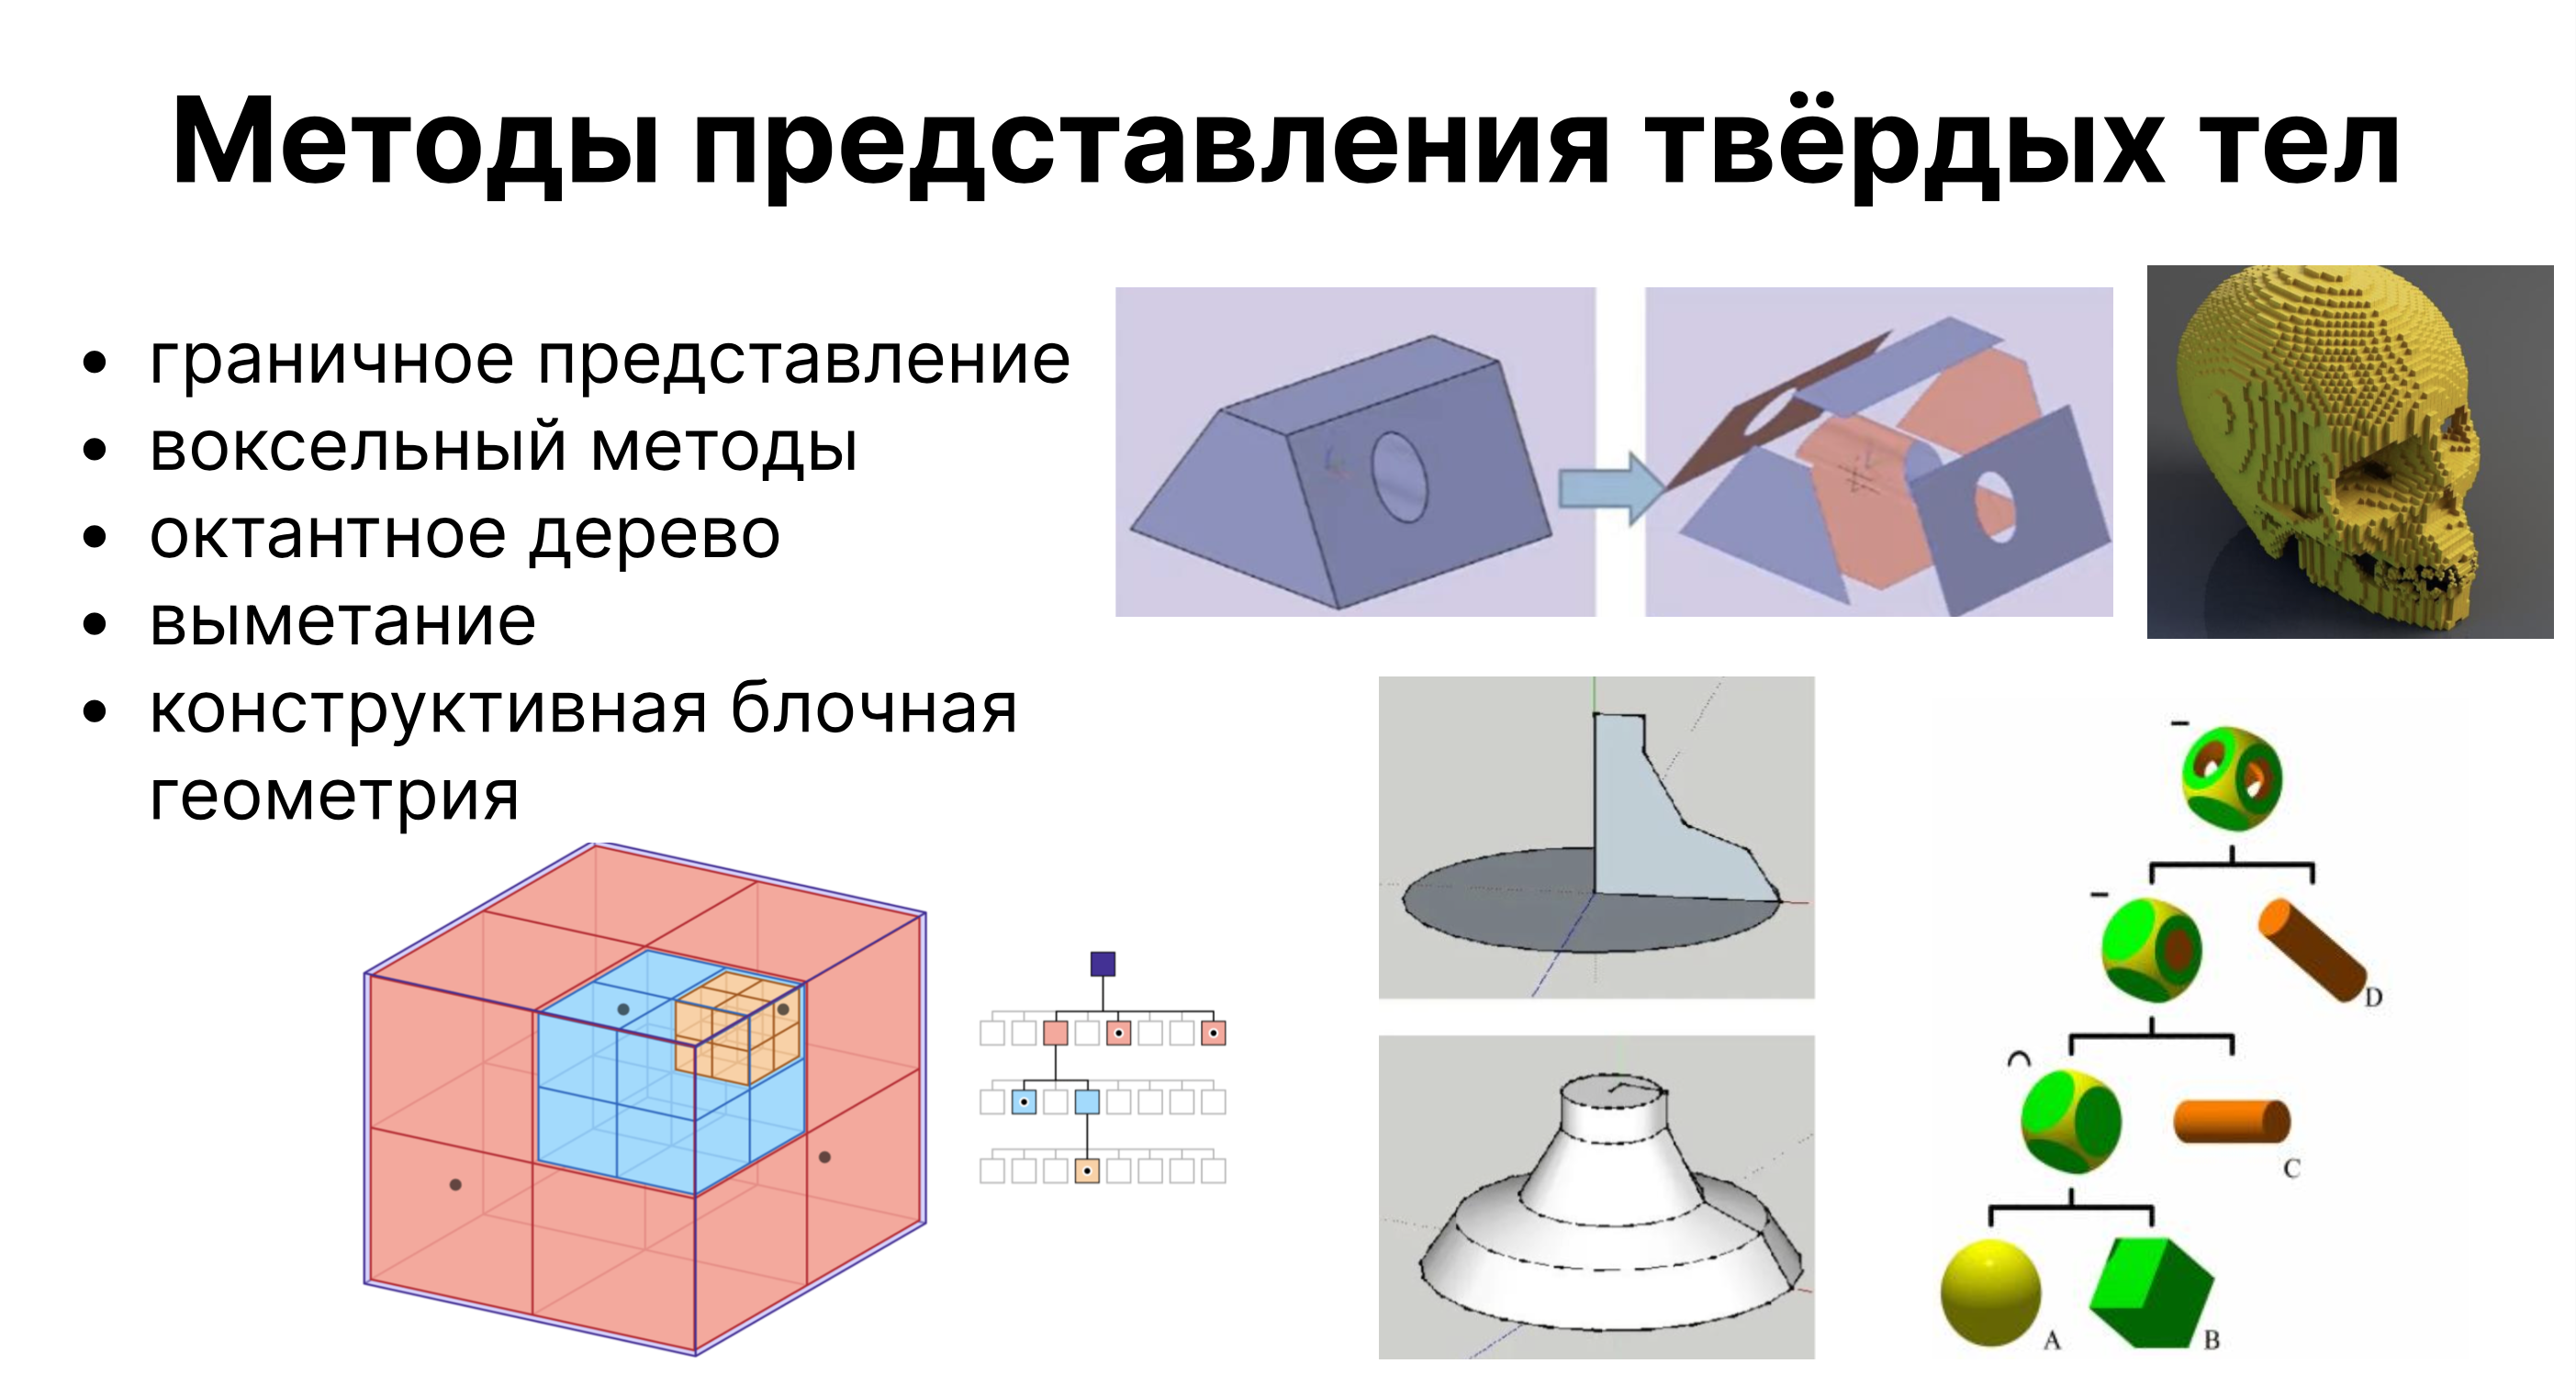
\includegraphics[width=150mm]{img/slide4.png}
	\caption{Методы представления твёрдых тел (слайд 4)}
	\label{fig:slide-4}
\end{figure}

\begin{figure}[h]
	\centering
	\captionsetup{justification=centering}
	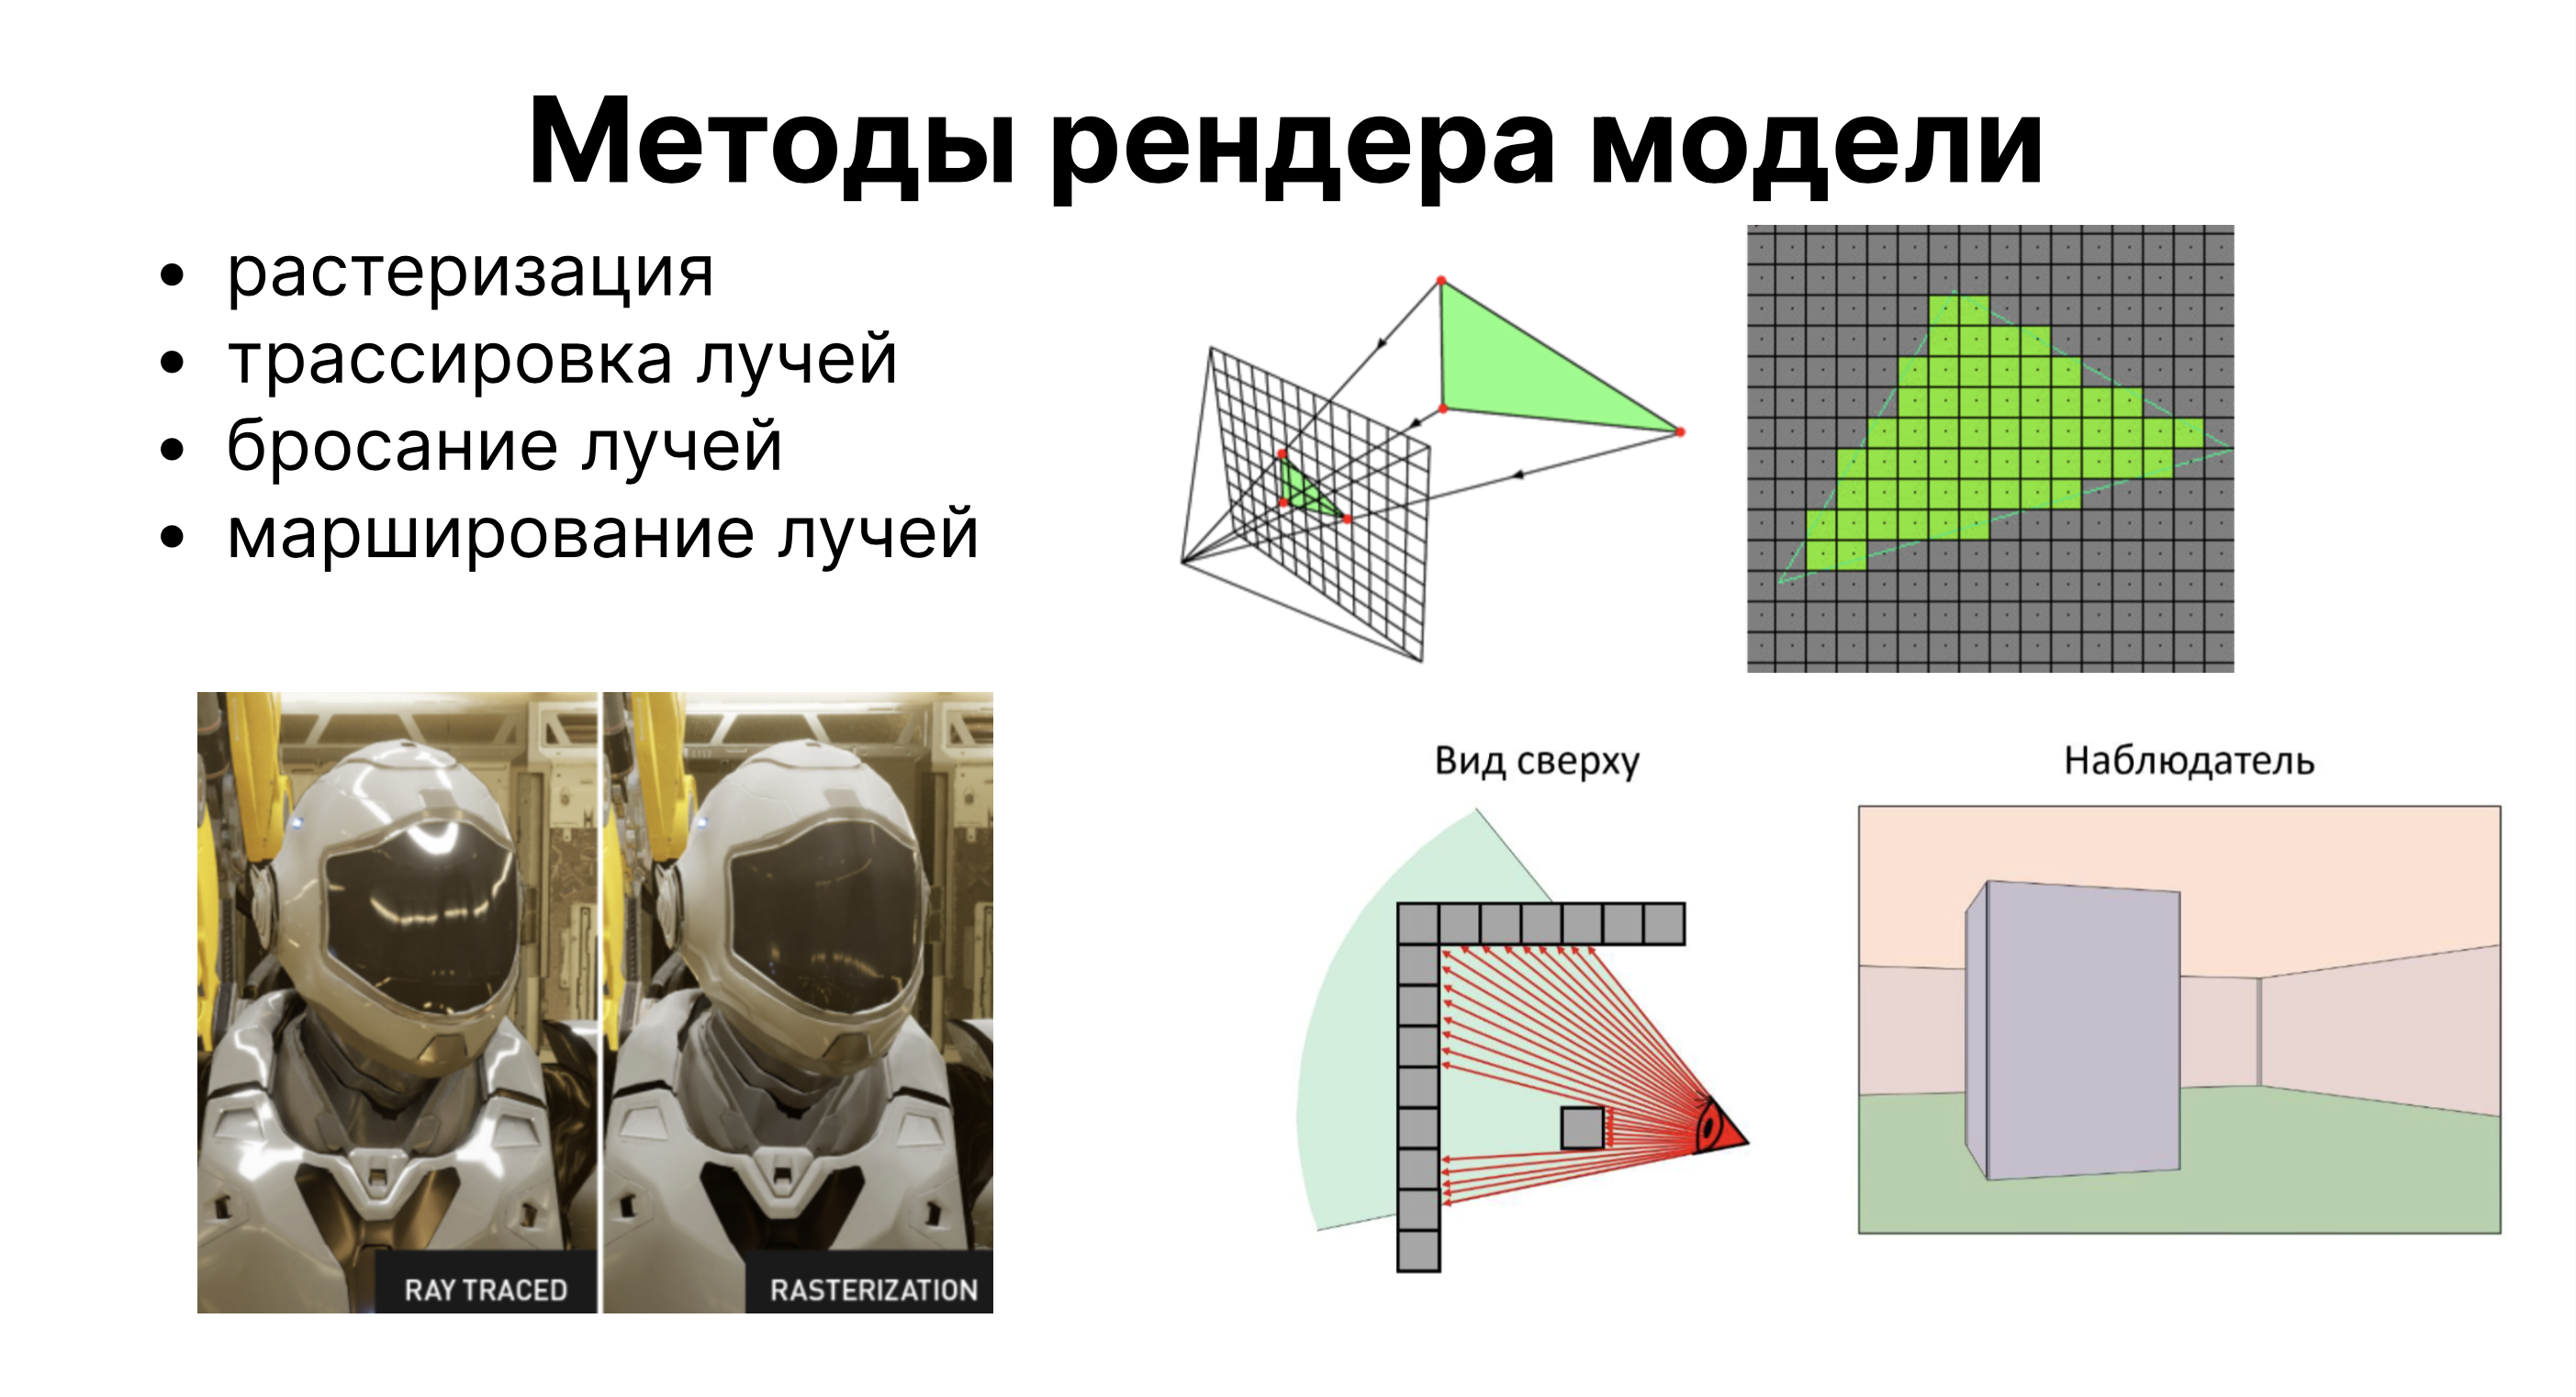
\includegraphics[width=150mm]{img/slide5.png}
	\caption{Методы рендера модели (слайд 5)}
	\label{fig:slide-5}
\end{figure}

\begin{figure}[h]
	\centering
	\captionsetup{justification=centering}
	
\includegraphics[width=150mm]{img/slide6.png}
	\caption{Методы преобразования и визуализации(слайд 6)}
	\label{fig:slide-6}
\end{figure}

\begin{figure}[h]
	\centering
	\captionsetup{justification=centering}
	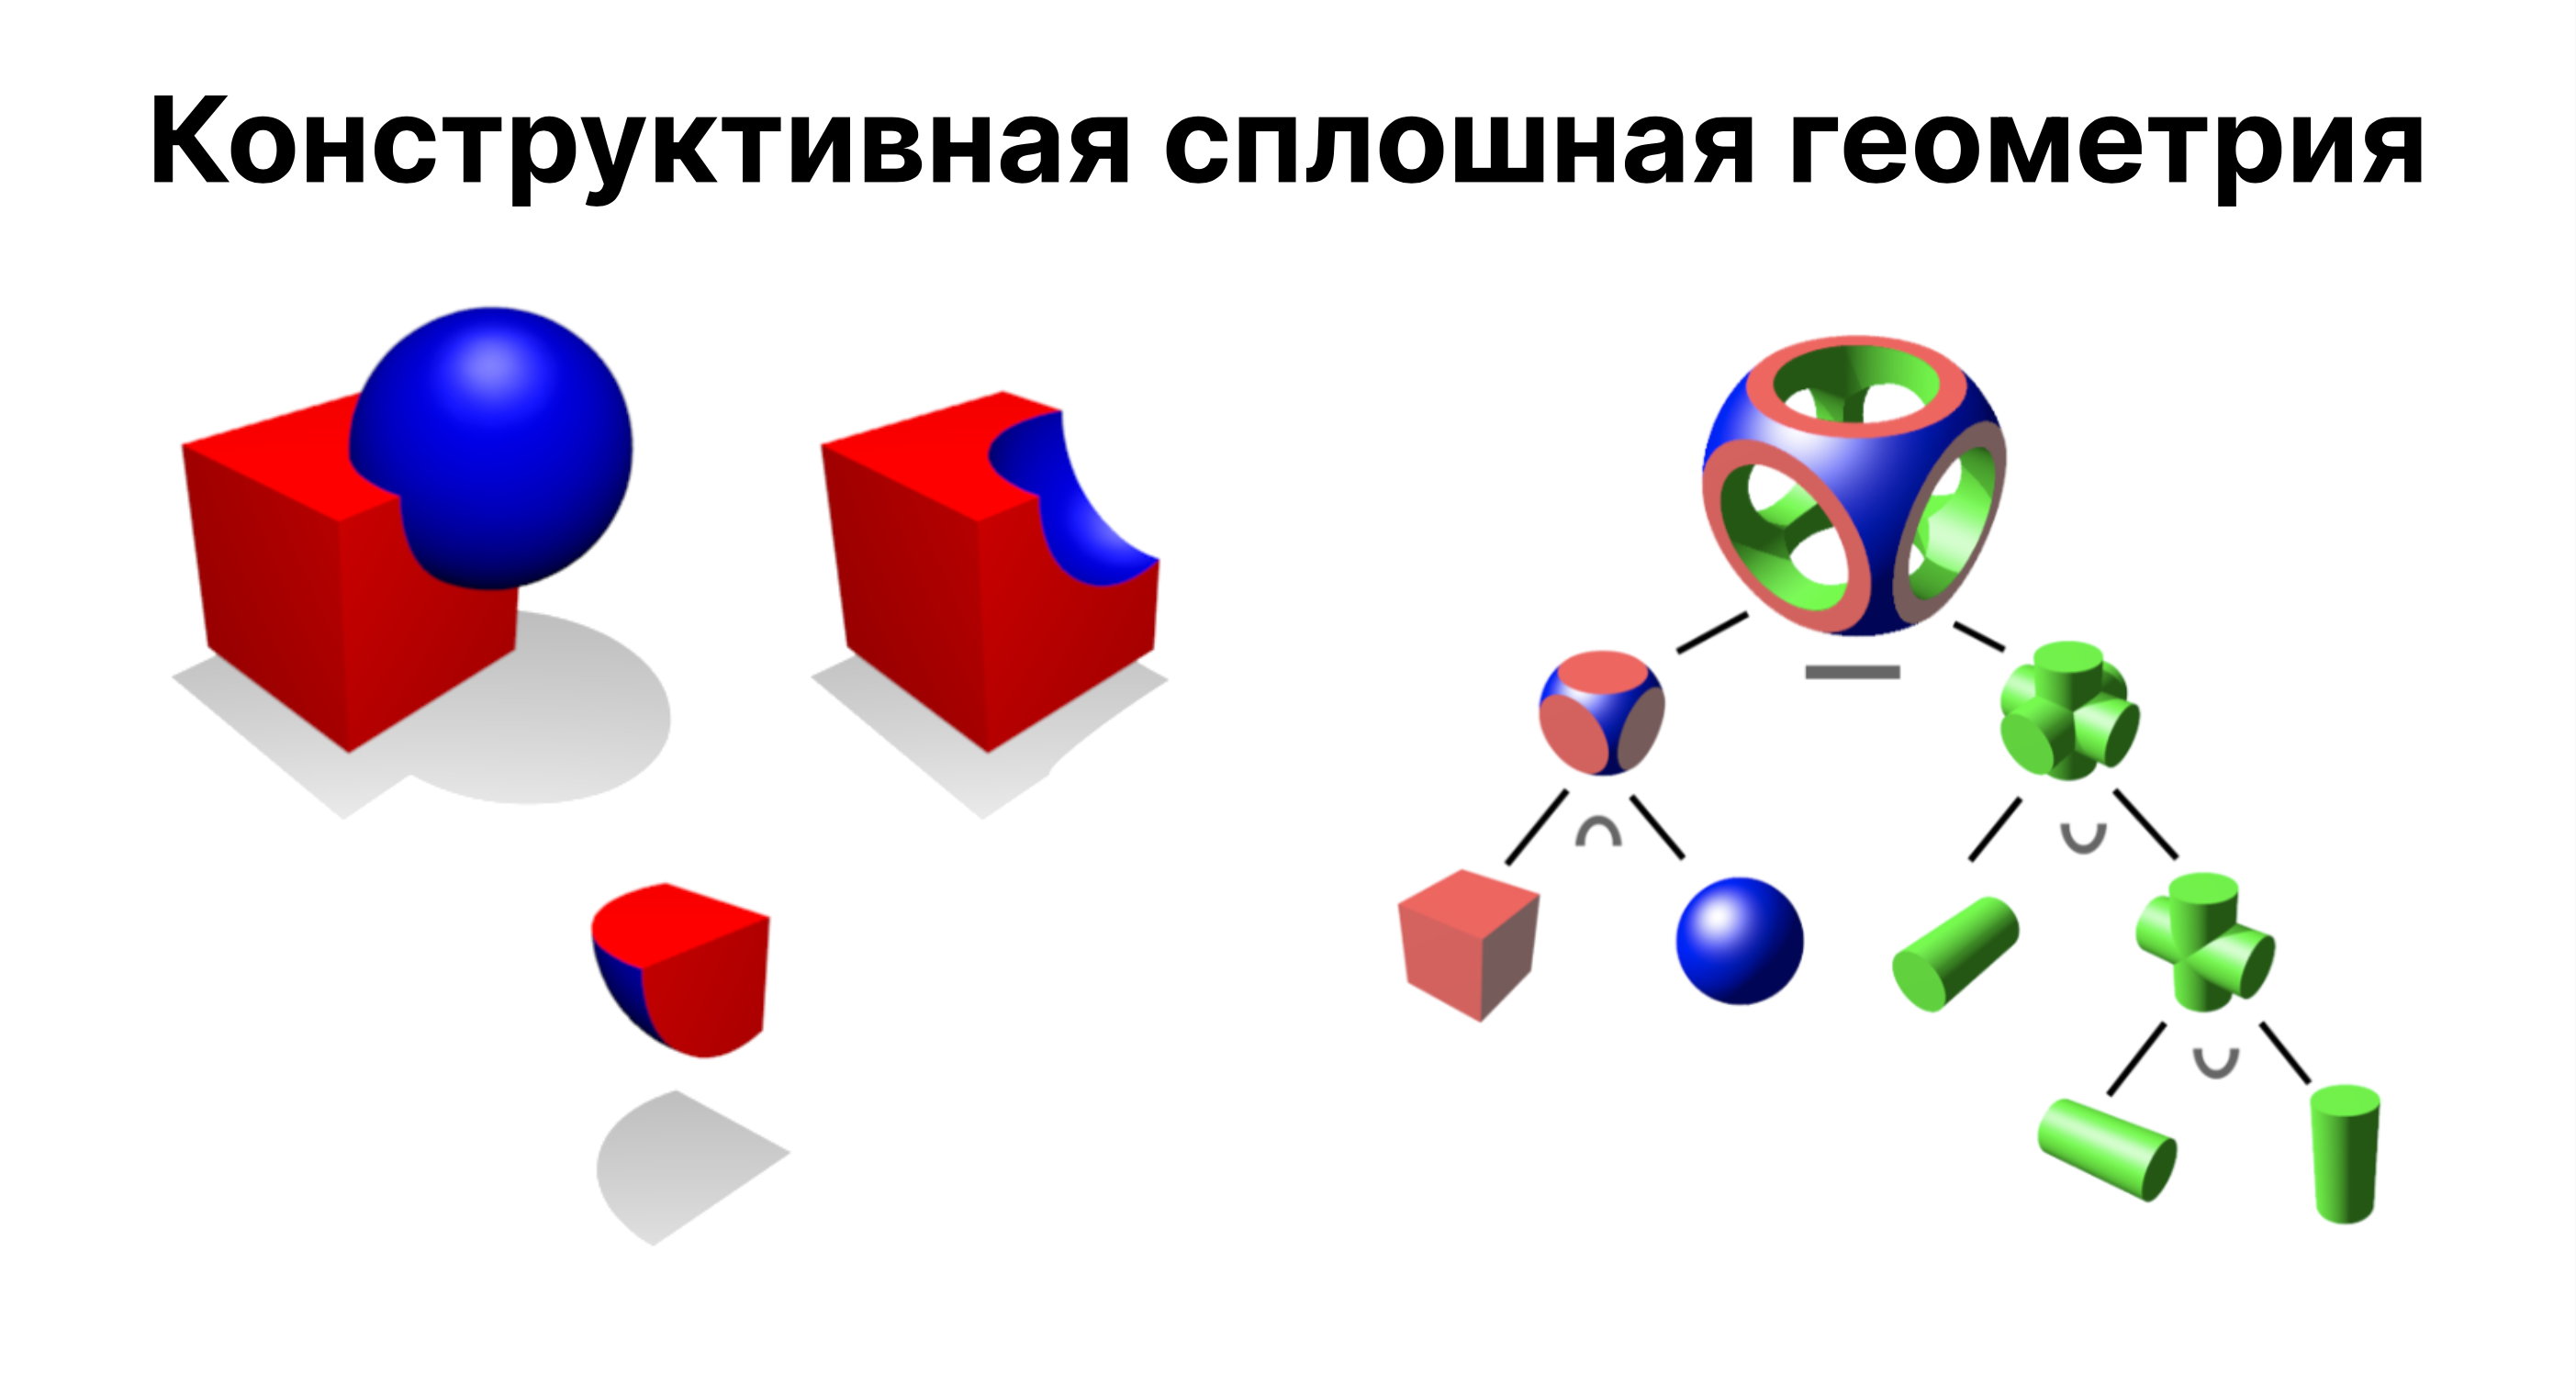
\includegraphics[width=150mm]{img/slide7.png}
	\caption{Конструктивная сплошная геометрия (слайд 7)}
	\label{fig:slide-7}
\end{figure}

\begin{figure}[h]
	\centering
	\captionsetup{justification=centering}
	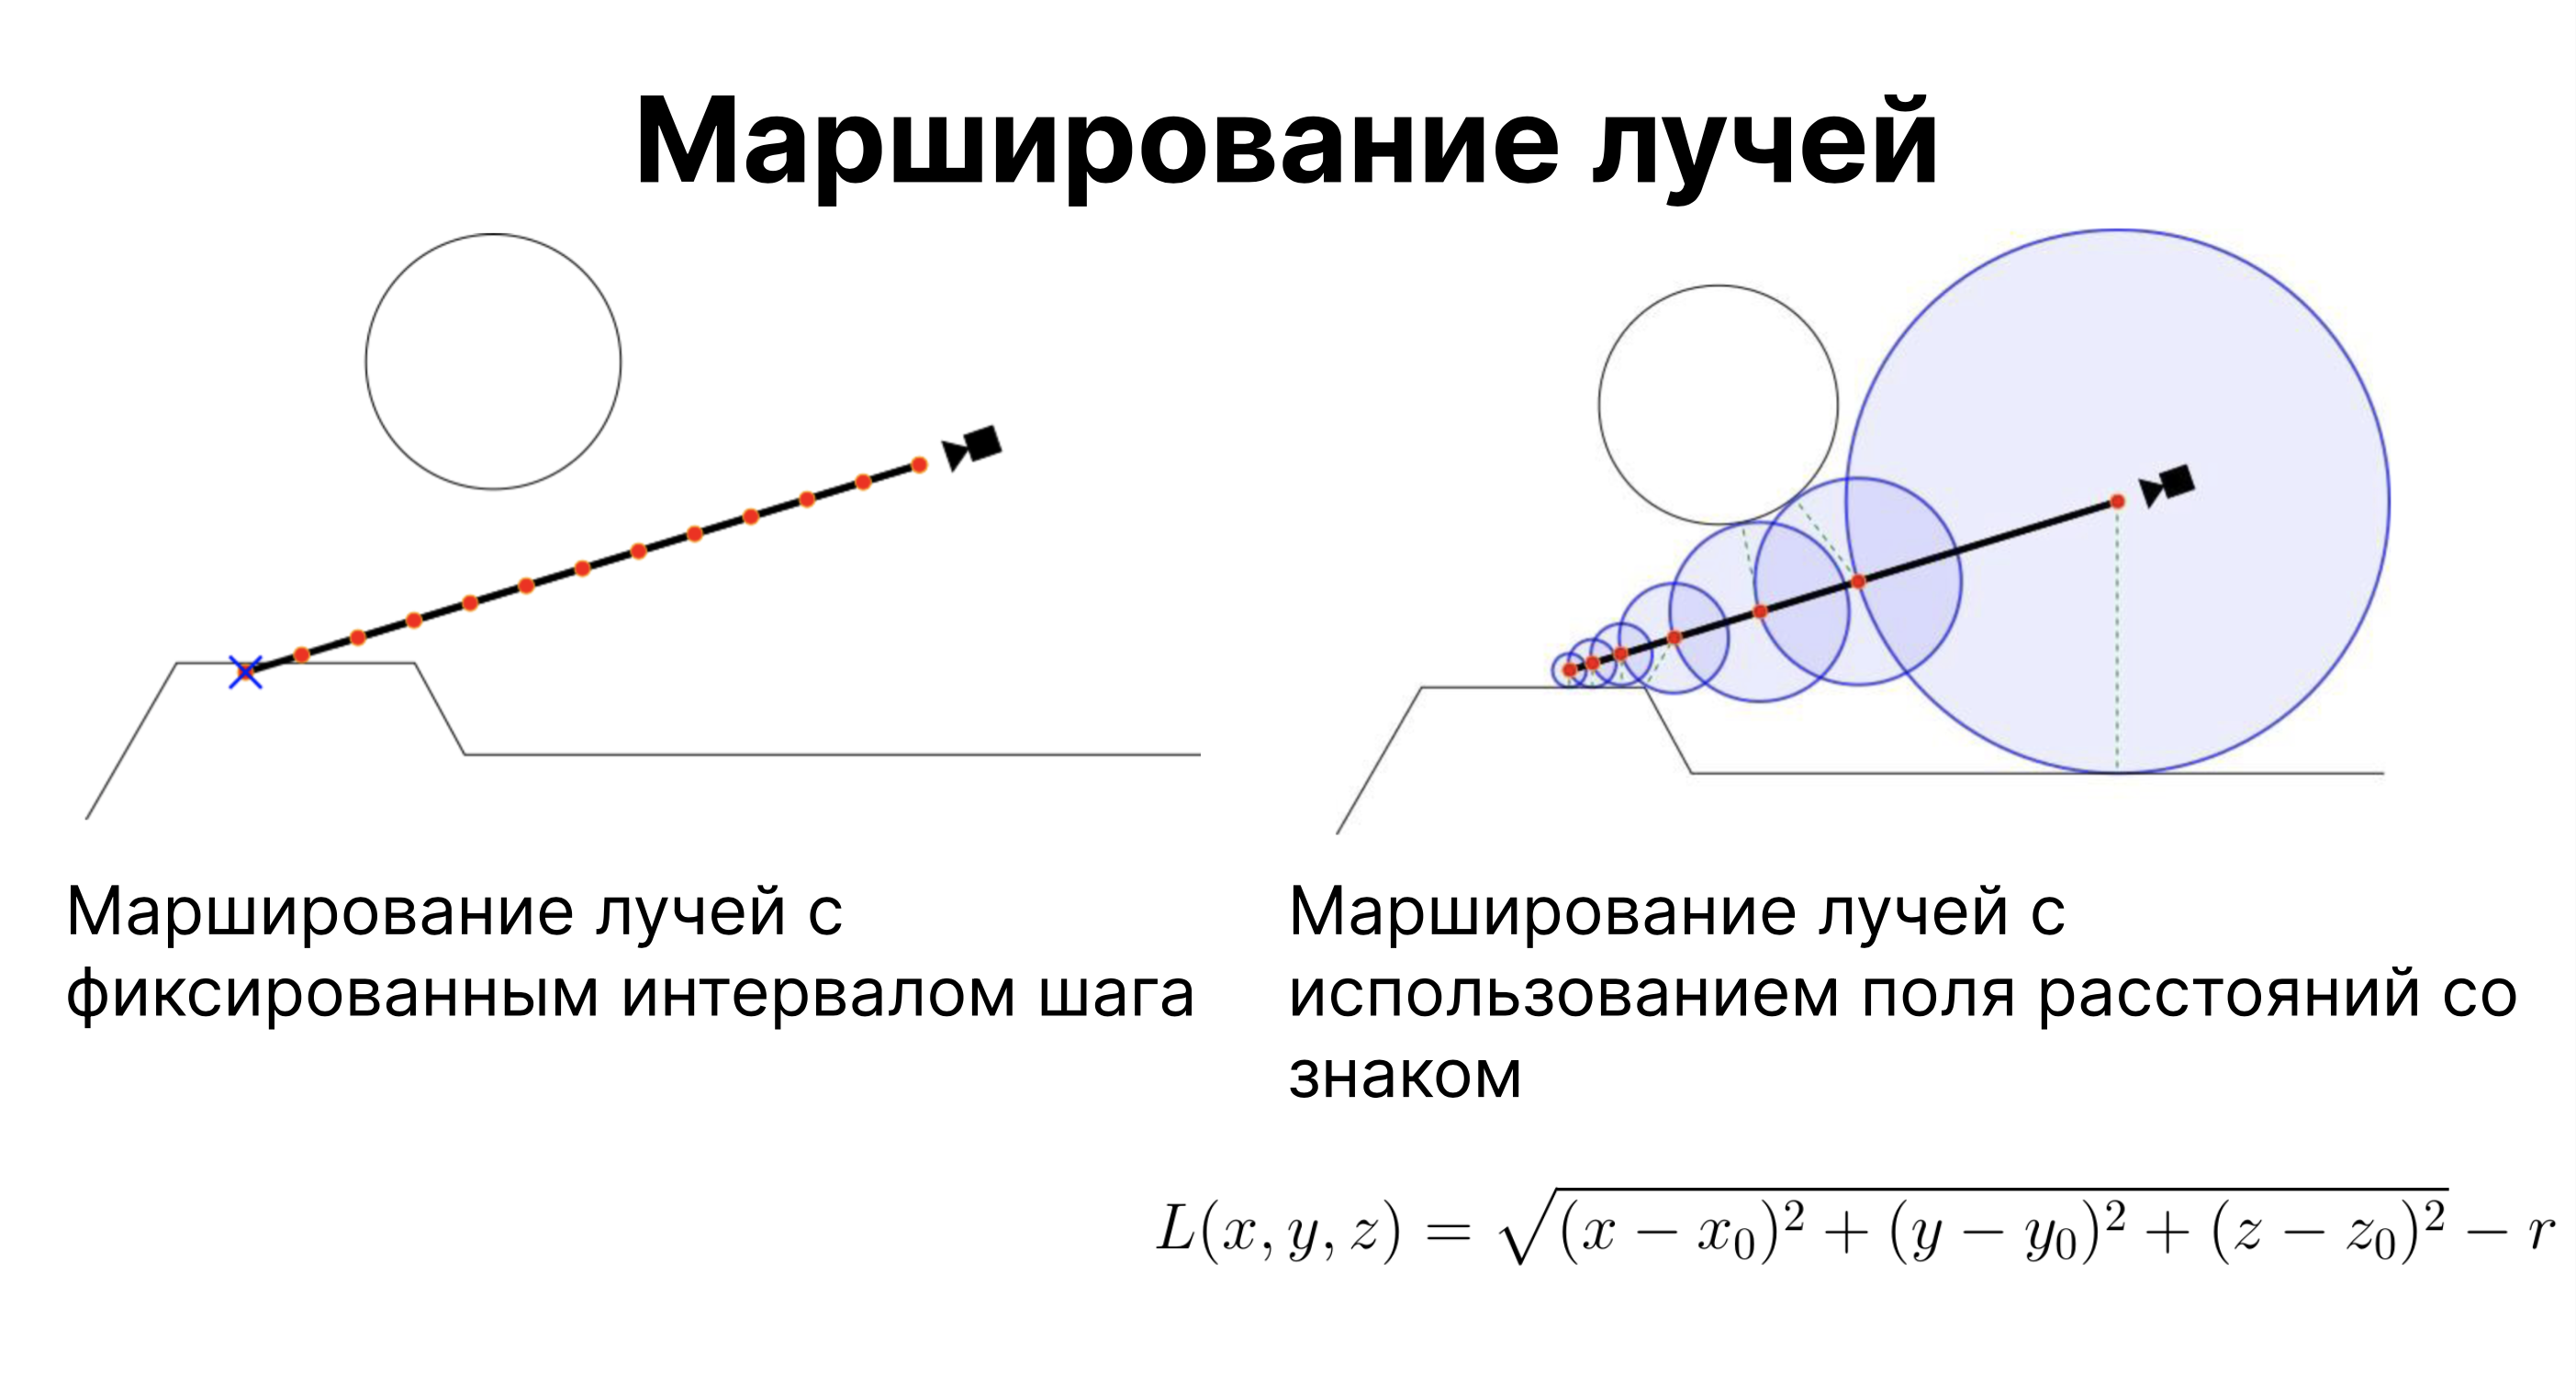
\includegraphics[width=150mm]{img/slide8.png}
	\caption{Марширование лучей (слайд 8)}
	\label{fig:slide-8}
\end{figure}

\begin{figure}[h]
	\centering
	\captionsetup{justification=centering}
	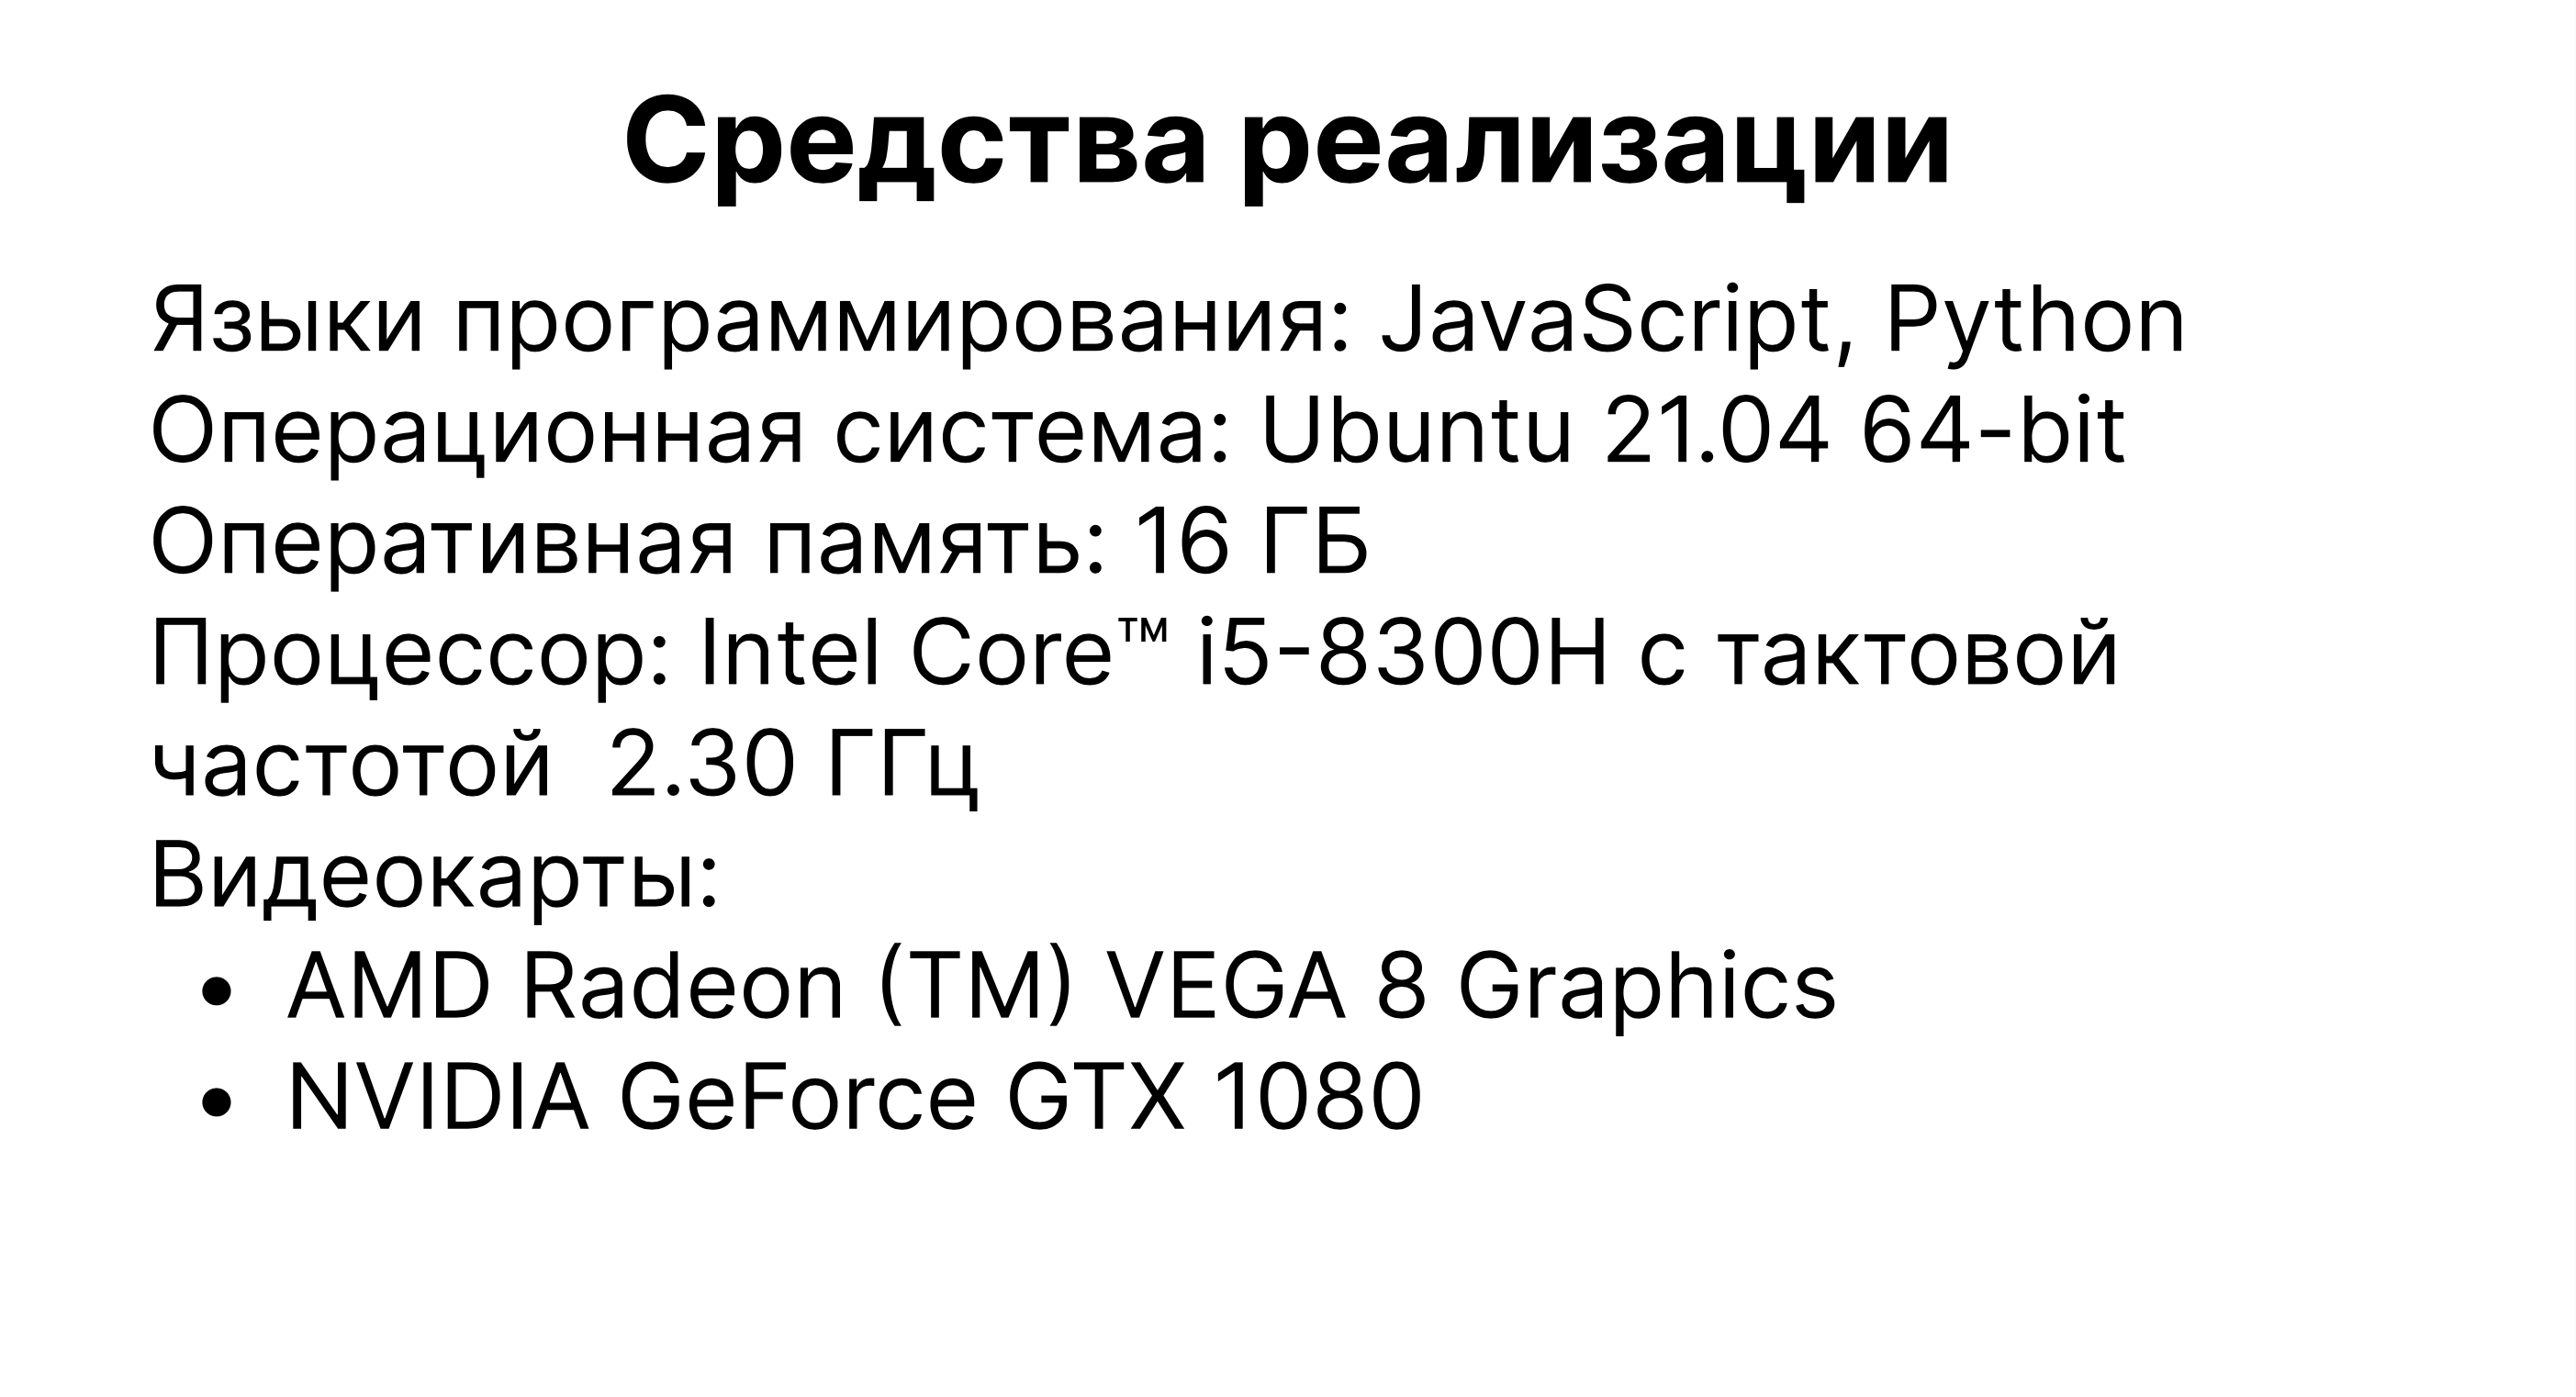
\includegraphics[width=150mm]{img/slide9.png}
	\caption{Средства реализации (слайд 9)}
	\label{fig:slide-9}
\end{figure}

\begin{figure}[h]
	\centering
	\captionsetup{justification=centering}
	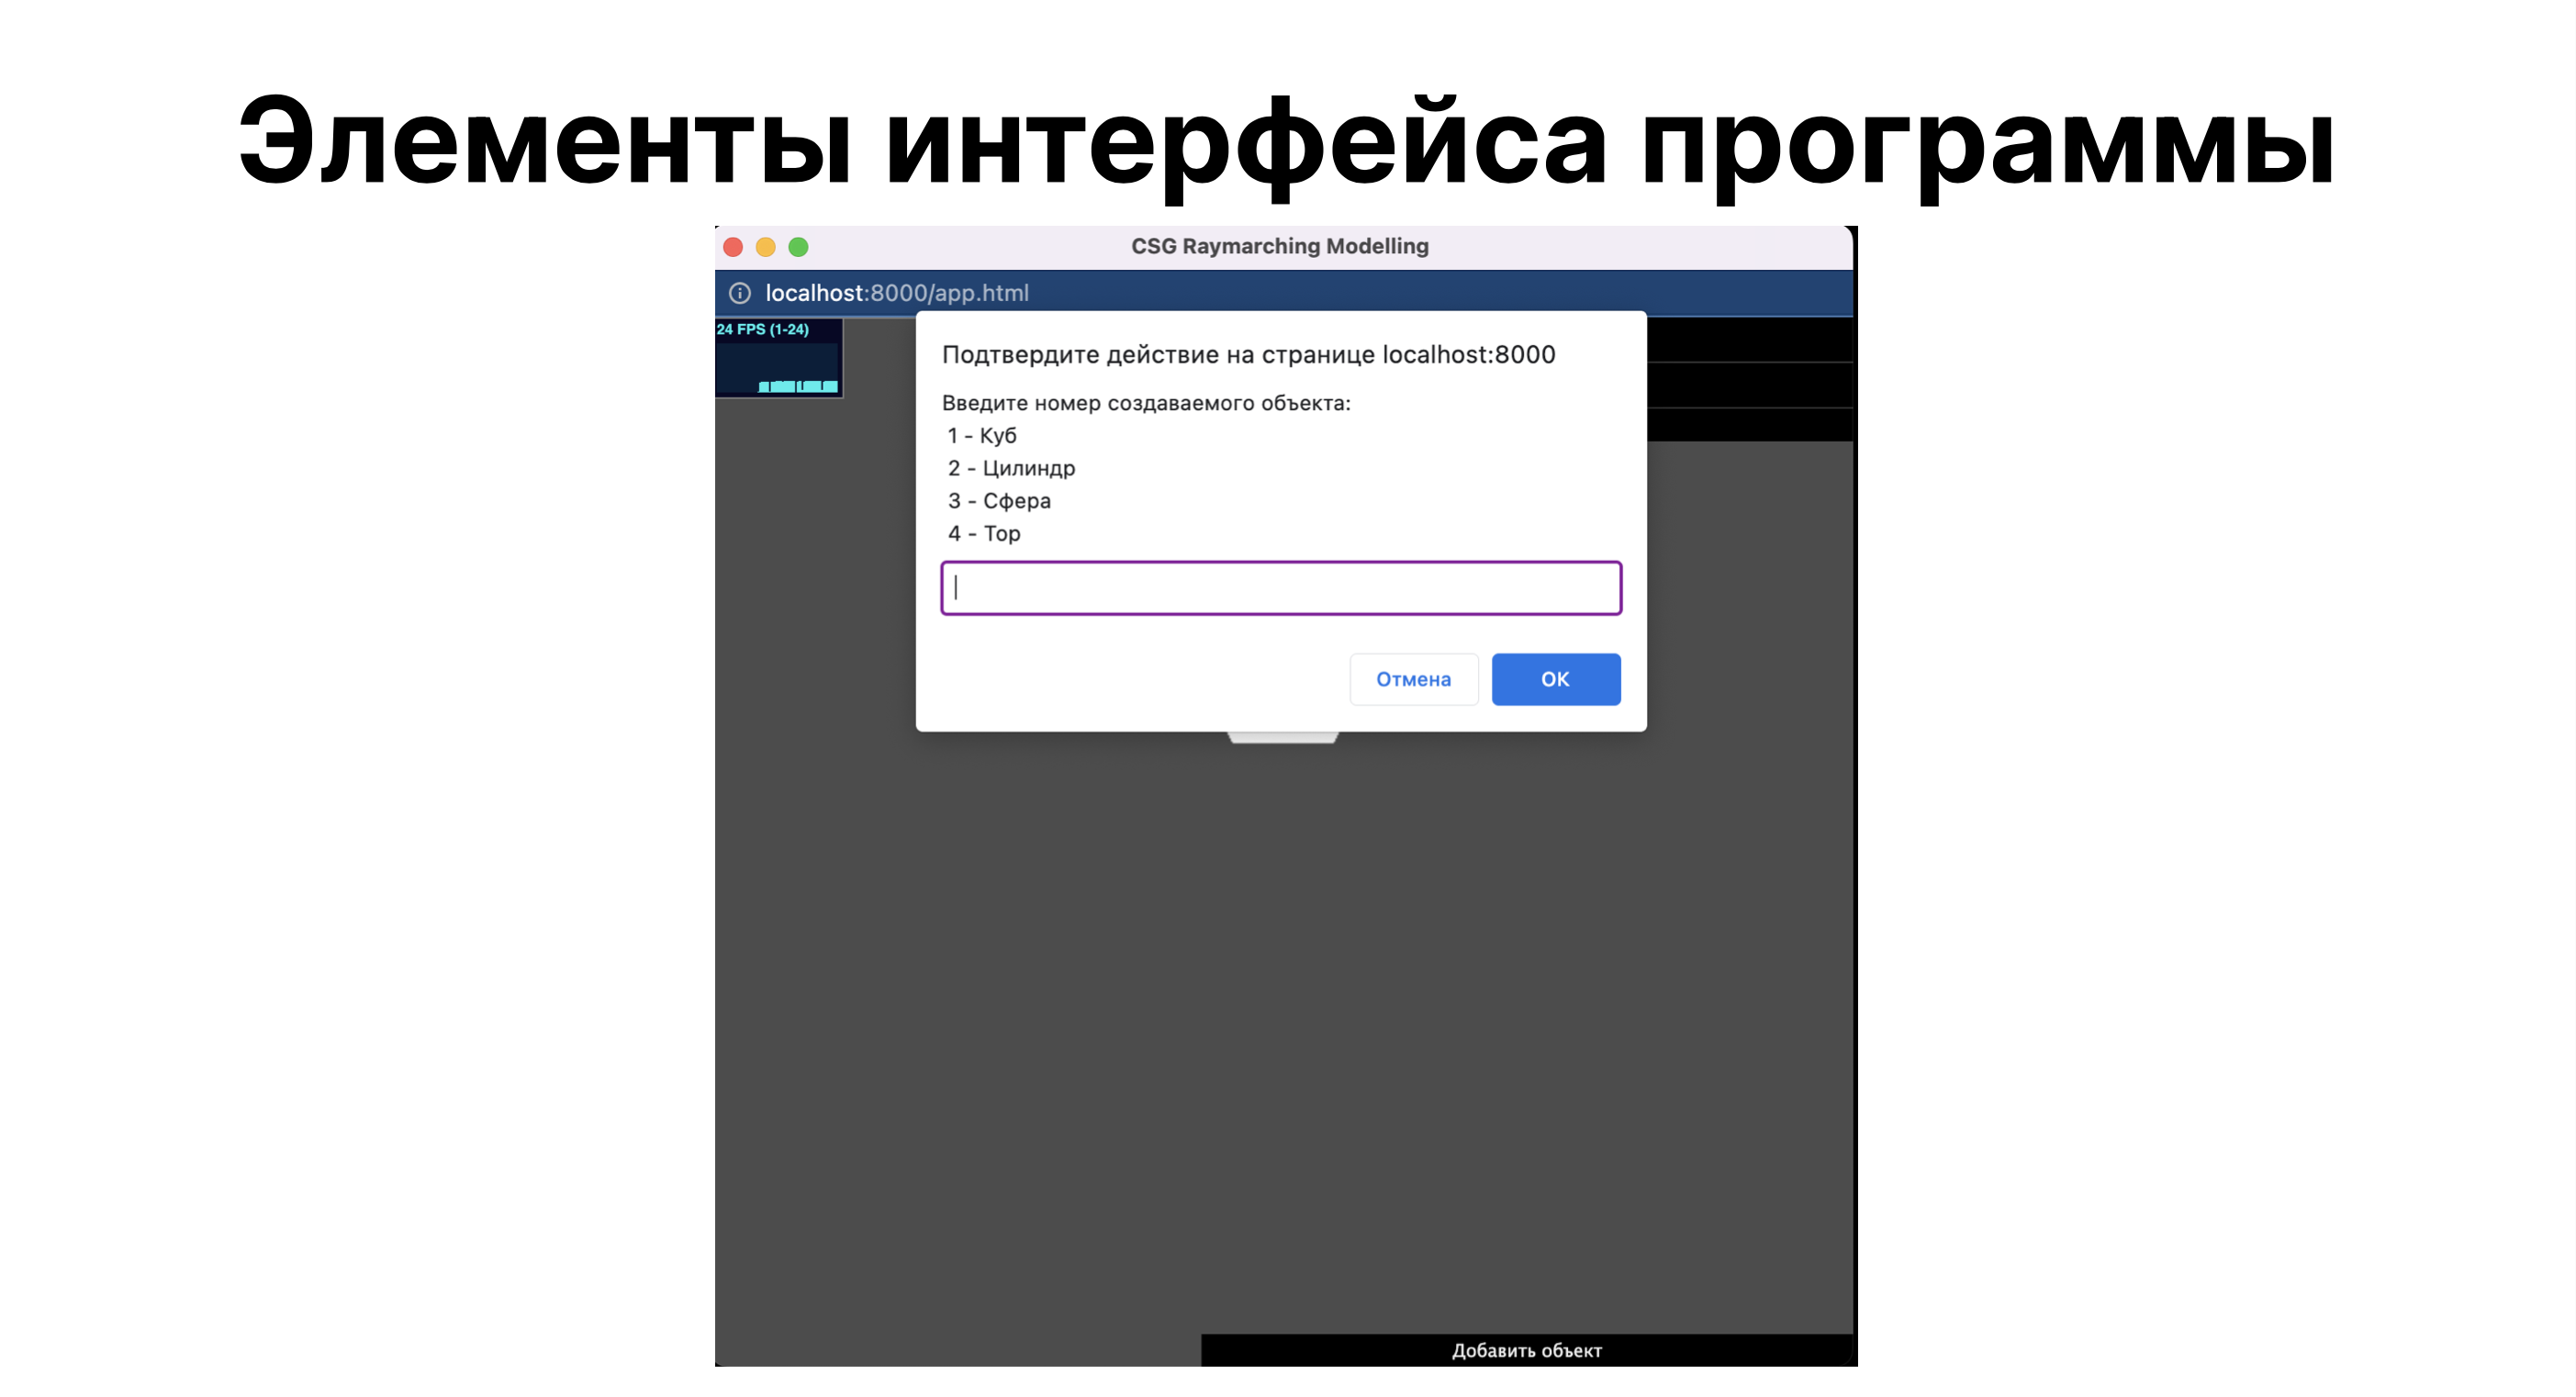
\includegraphics[width=150mm]{img/slide10.png}
	\caption{Элементы интерфейса программы, часть 1 (слайд 10)}
	\label{fig:slide-10}
\end{figure}

\begin{figure}[h]
	\centering
	\captionsetup{justification=centering}
	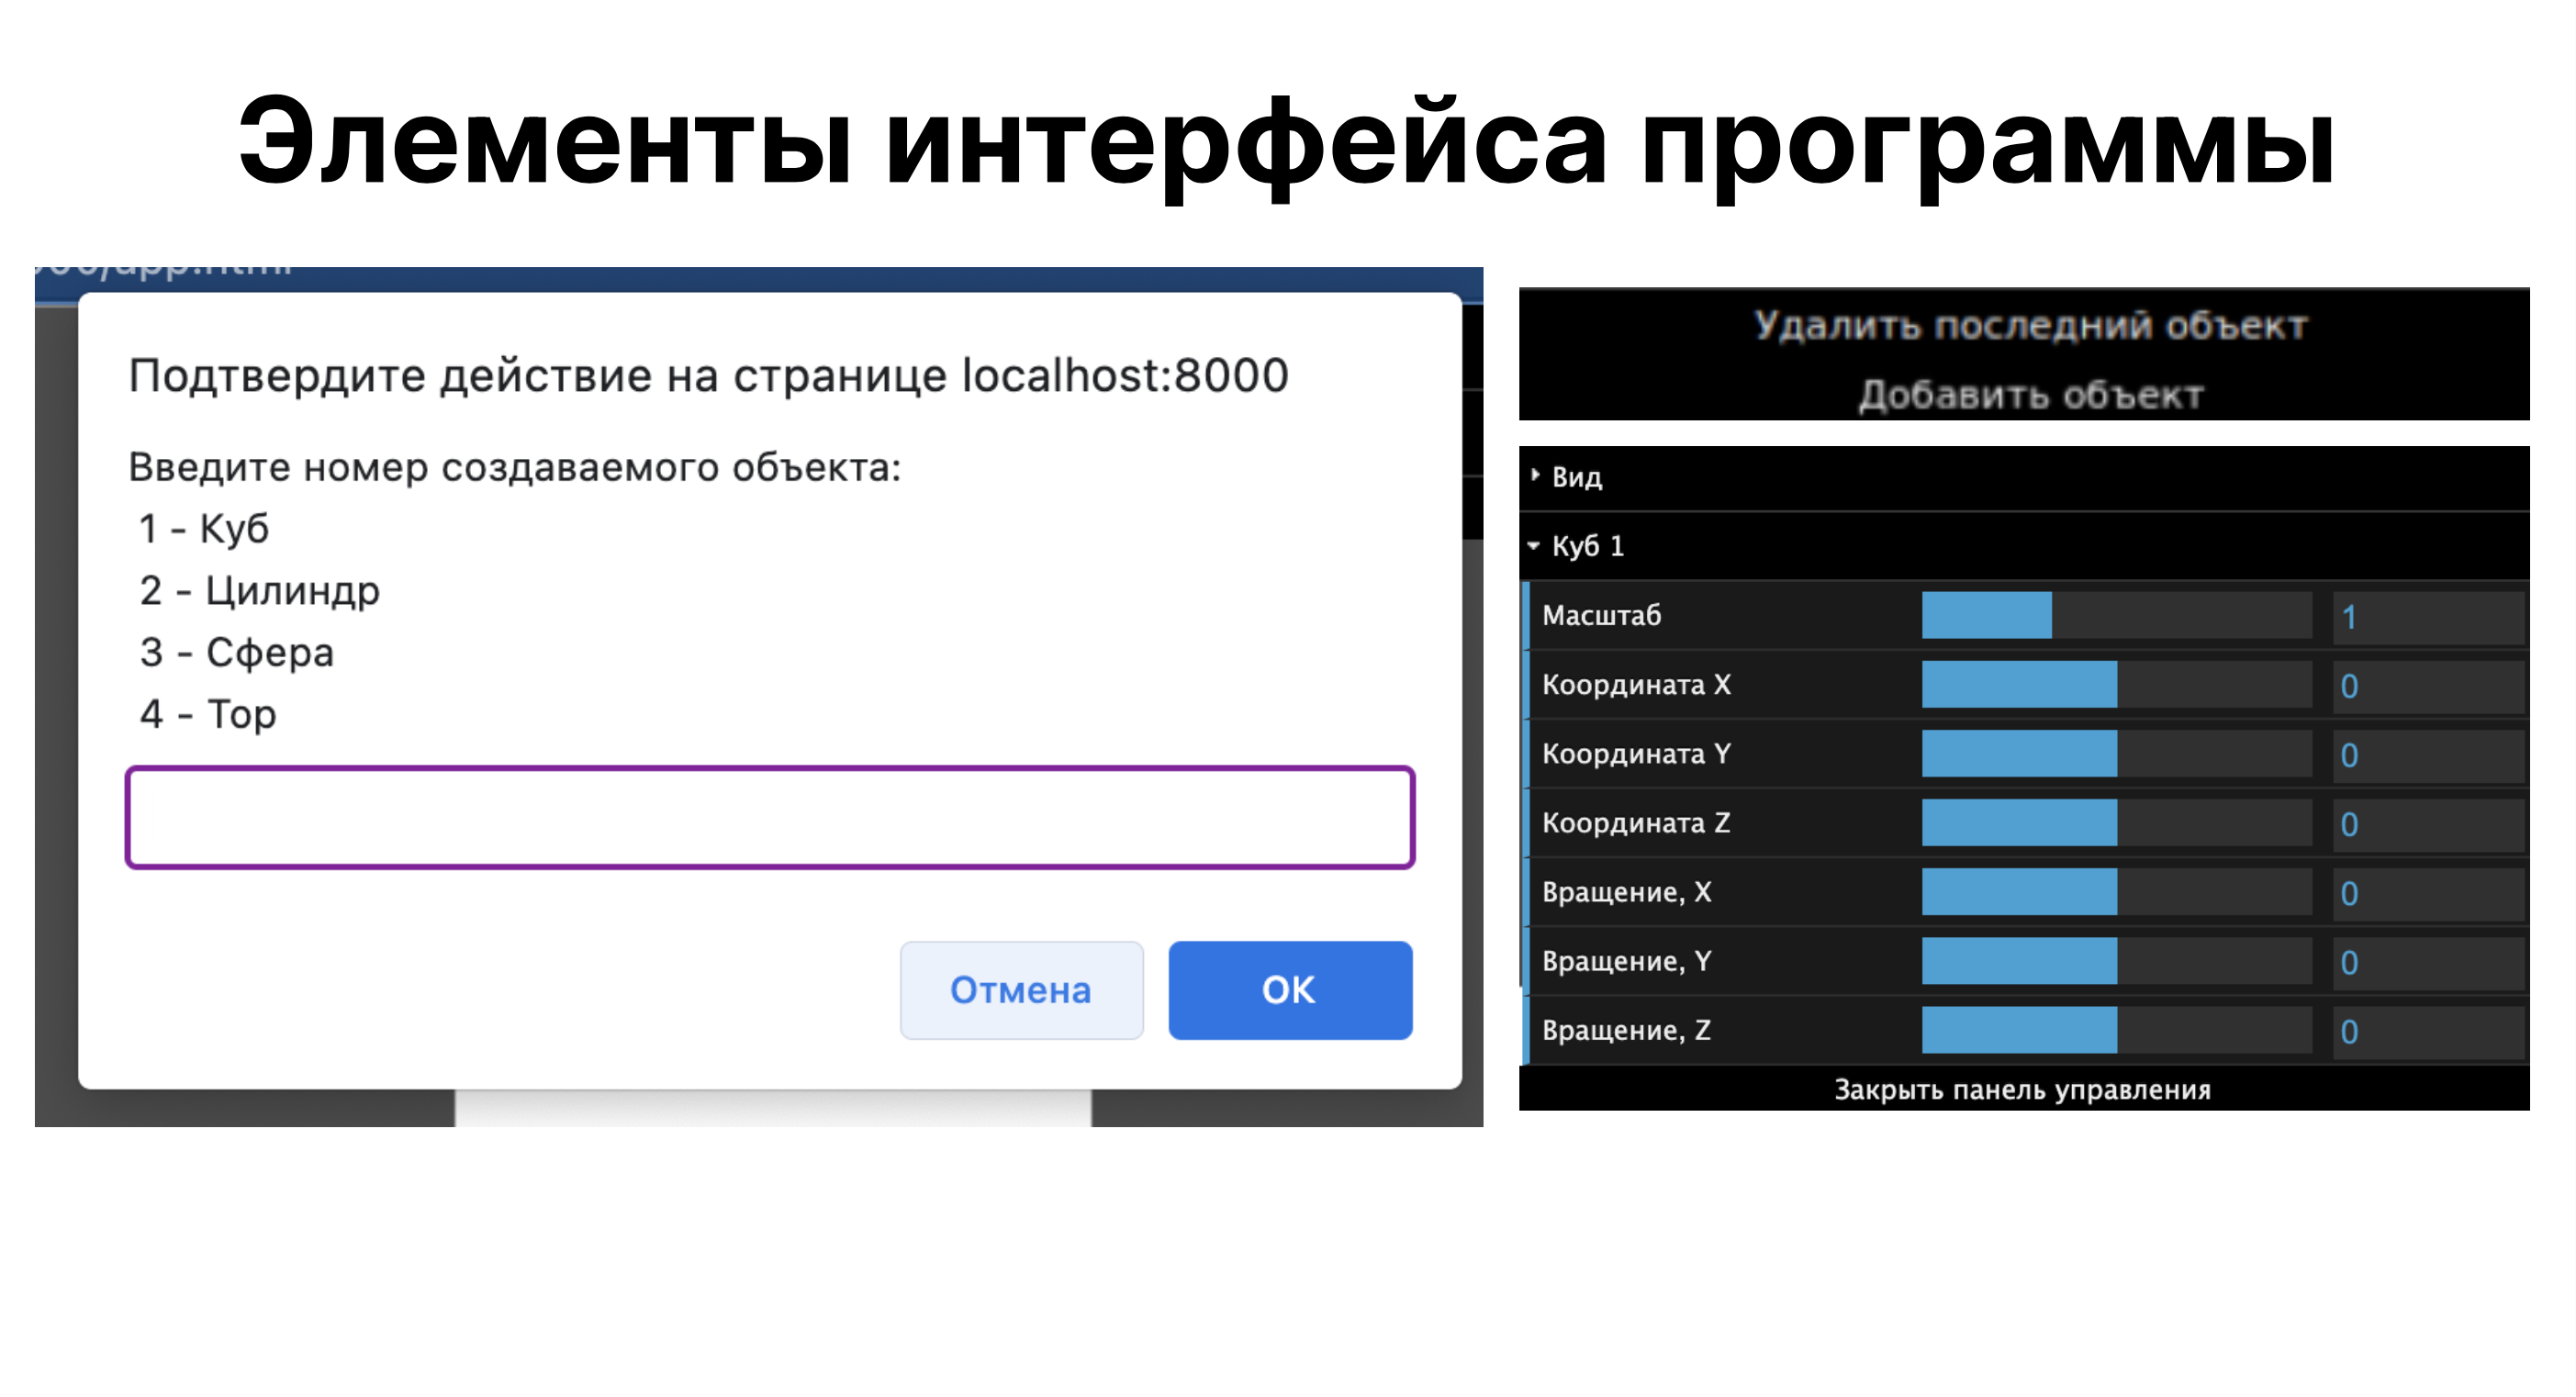
\includegraphics[width=150mm]{img/slide11.png}
	\caption{Элементы интерфейса программы, часть 2 (слайд 11)}
	\label{fig:slide-11}
\end{figure}

\begin{figure}[h]
	\centering
	\captionsetup{justification=centering}
	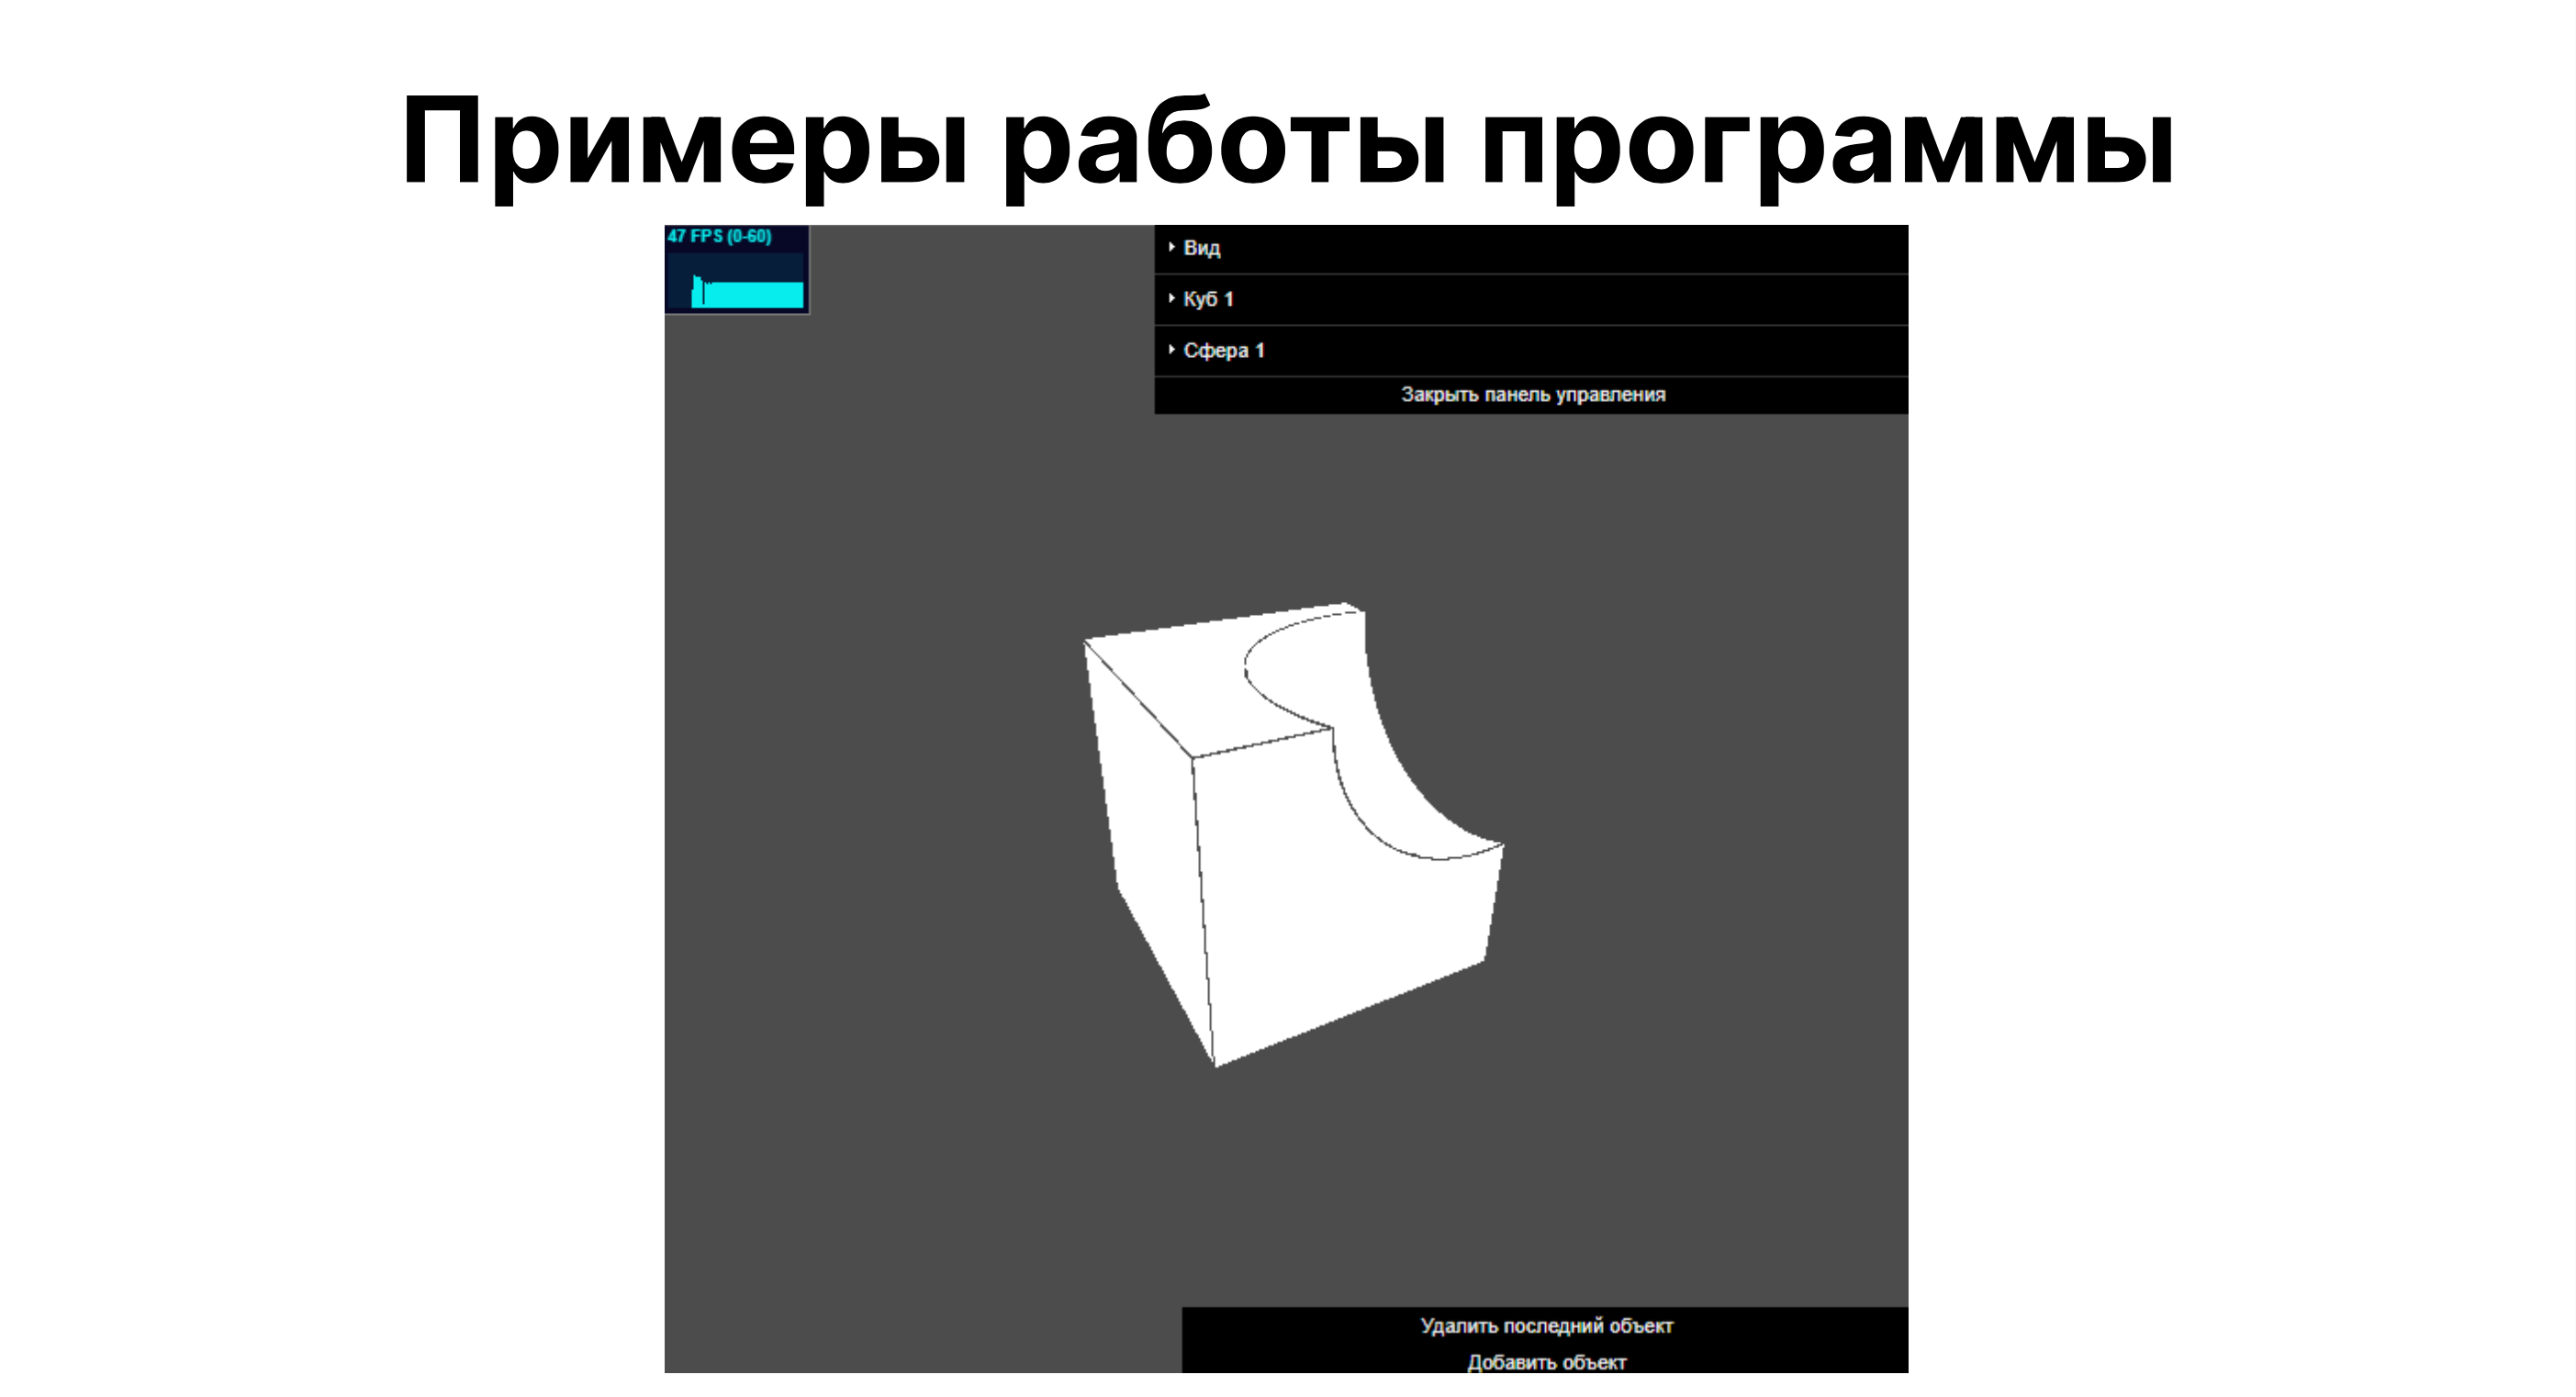
\includegraphics[width=150mm]{img/slide12.png}
	\caption{Пример работы программы, часть 1 (слайд 12)}
	\label{fig:slide-12}
\end{figure}

\begin{figure}[h]
	\centering
	\captionsetup{justification=centering}
	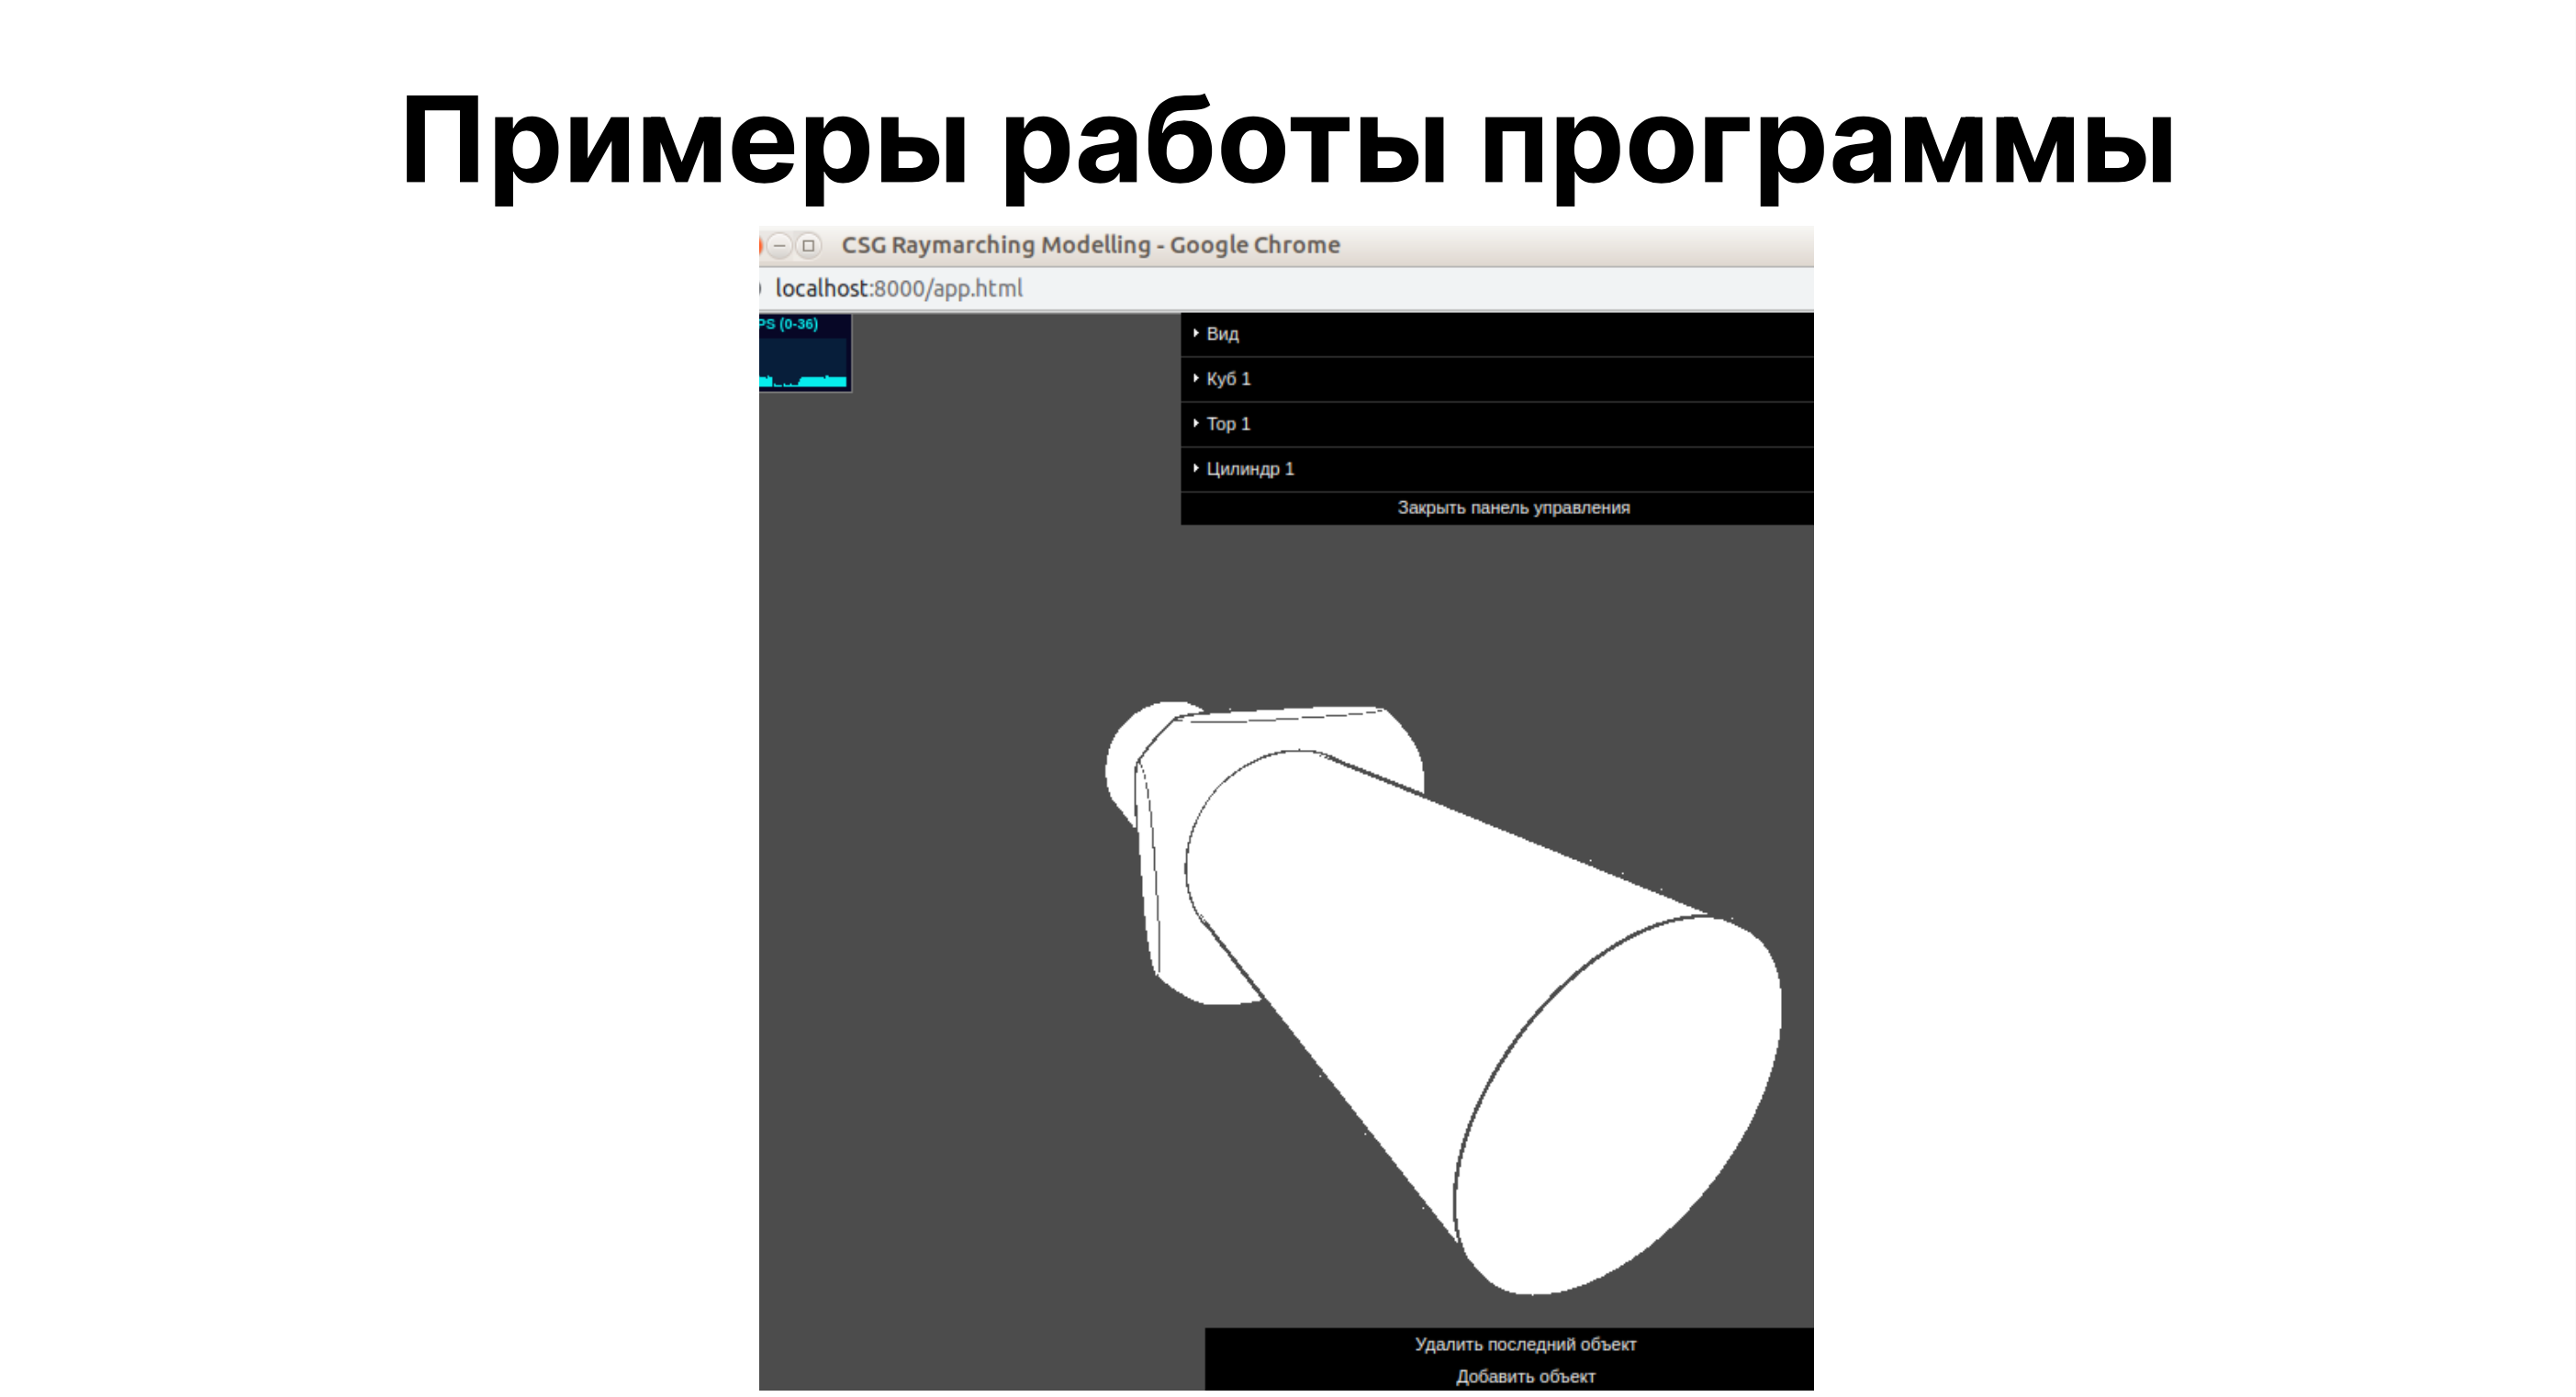
\includegraphics[width=150mm]{img/slide13.png}
	\caption{Пример работы программы, часть 2 (слайд 13)}
	\label{fig:slide-13}
\end{figure}

\begin{figure}[h]
	\centering
	\captionsetup{justification=centering}
	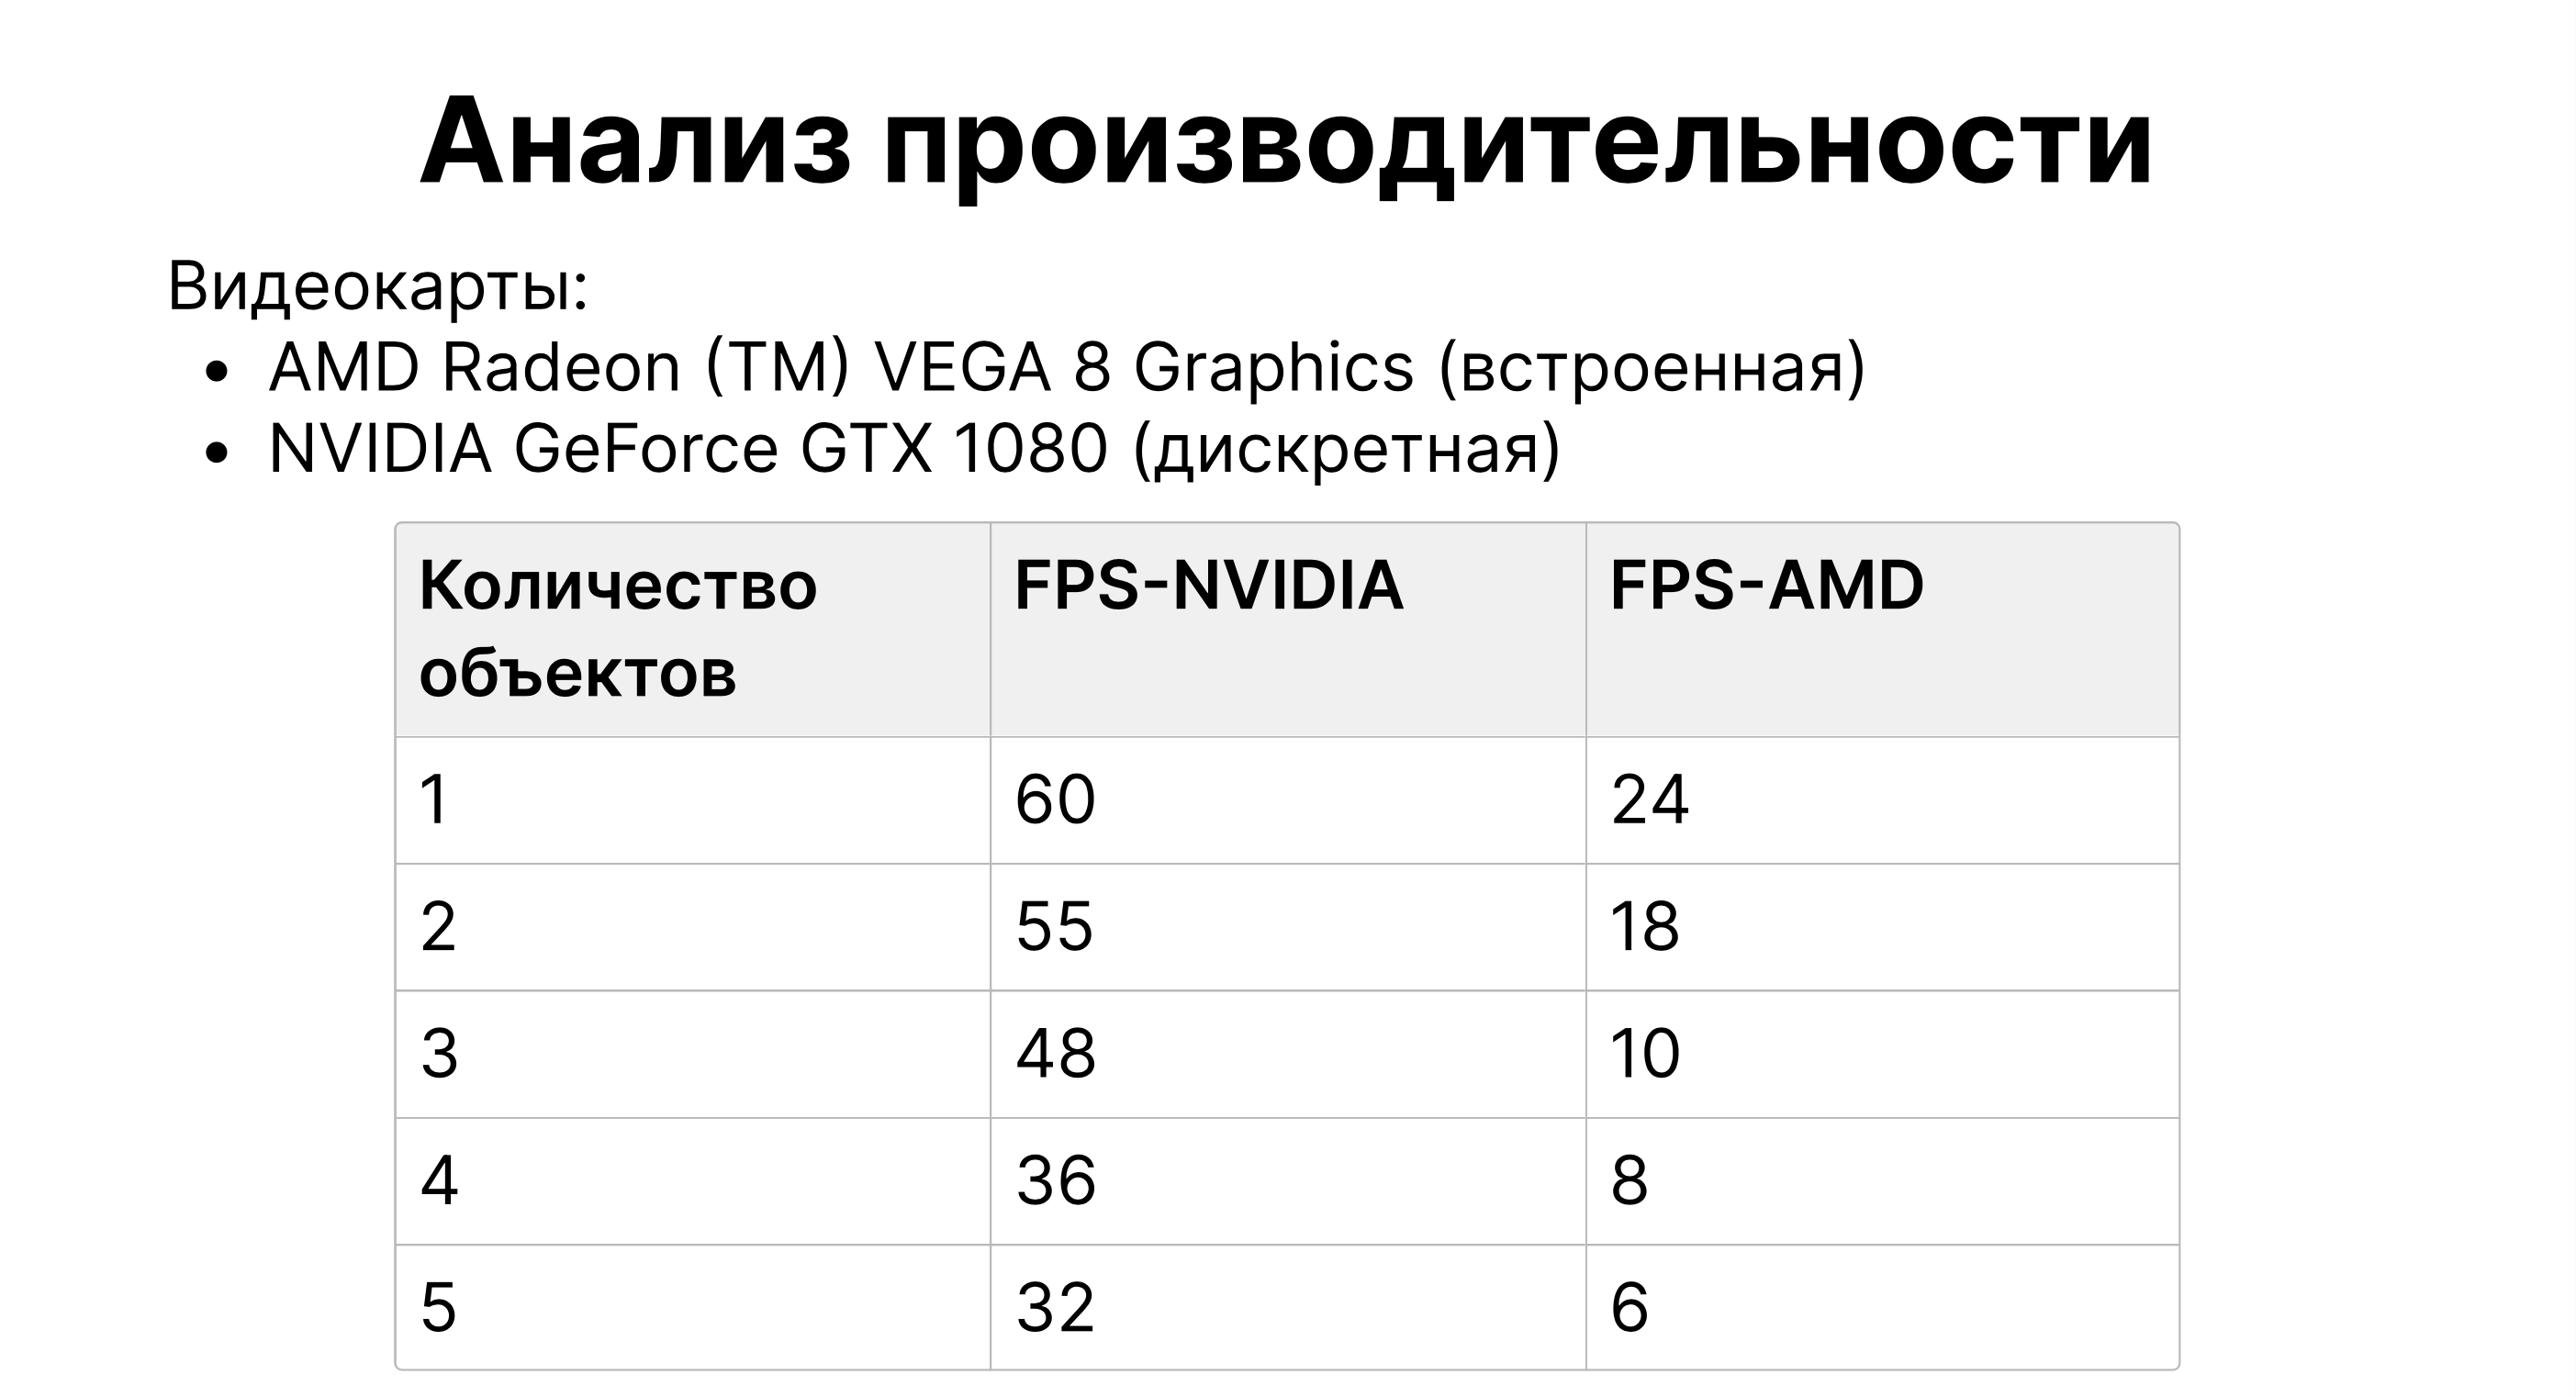
\includegraphics[width=150mm]{img/slide14.png}
	\caption{Анализ производительности (слайд 14)}
	\label{fig:slide-14}
\end{figure}

\begin{figure}[h]
	\centering
	\captionsetup{justification=centering}
	
\includegraphics[width=150mm]{img/slide15.png}
	\caption{Заключение (слайд 15)}
	\label{fig:slide-15}
\end{figure}
\pagebreak